% This is file JFM2esam.tex
% first release v1.0, 20th October 1996
%       release v1.01, 29th October 1996
%       release v1.1, 25th June 1997
%       release v2.0, 27th July 2004
%       release v3.0, 16th July 2014
%       release v4.0, 15th June 2017
%   (based on JFMsampl.tex v1.3 for LaTeX2.09)
% Copyright (C) 1996, 1997, 2014, 2017 Cambridge University Press

% Outline and section completion
% - Magnetic probes
%   - [x] Magnetic field probes
%   - [x] Rogowski coils
% - Electric probes
%   - [x] Langmuir Probes
%   - [x] Gridded energy analyzers
% - Line radiation spectroscopy
%   - [x] ChERS
%   - [x] LIF/TALIF
%   - [x] [x] [x] Zeeman spectroscopy
% - Scattering of EM radiation
%   - [x] Coherent Thomson scattering
%   - [x] Incoherent Thomson scattering
% - Imaging
%   - [x] Coded aperture imaging
%   - [x] IR imaging / two-color pyrometry
% - Polarimetry
%   - [ ] Pulsed Polarimetry
%   - [x] VISAR
% - Fusion products
%   - [x] Neutron Diagnostics
% - Ex Situ Diagnostics
%   - [x] XPS

% Done: 16/19
% Fri
%  - [x] magnetic field probes
%  - [x] rogowski coils
% Sat
%  - [x] neutron diagnostics
%  - [x] ChERS
% Sun
%  - [x] lif/talif
%  - [X] XPS
% Mon
%  - [x] IR/two-color pyrometry
%  - [x] coded aperture imaging
% Tue
%  - [x] incoherent thomson
%  - [x] langmuir probes
% Wed
%  - [x] Zeeman spectroscopy (THE BIG ONE)
% Thu
%  - [x] coherent thomson
%  - [x] visar
% Fri
%  - [x] gridded energy analyzer
%  - [ ] pulsed polarimetry
%  - [ ] introduction
%  - [ ] review


\documentclass{jpp}
\usepackage{graphicx}
% \usepackage{epstopdf, epsfig}

\usepackage[utf8]{inputenc}
\usepackage[T1]{fontenc}
\usepackage{amsmath}
\usepackage{physics}
\newcommand{\angstrom}{\text{\normalfont\AA}}

\shorttitle{Summary of Plasma Diagnostic Methods}
\shortauthor{Summary of Plasma Diagnostic Methods}

\title{Summary of Plasma Diagnostic Methods}

\author{Evan Bluhm}
% \aff{1}
%   \corresp{\email{jpp@damtp.cam.ac.uk}},
%   H. - C. Smith\aff{1}
%  \and J. Q.  Public\aff{2}}

\begin{document}

\maketitle

\section{Introduction}



\section{Magnetic Field Diagnostics}

\subsection{B-dot Field Probes}

The simplest magnetic field measurement is obtained by straightforward application of Faraday's law to a loop of conducting wire. Assuming an open circuit, a changing magnetic field will induce a voltage $V_{emf}$ :
\begin{equation*}
\int_{area} \pdv{\vec B}{t} \cdot \dd \vec S = - \oint _{loop} \vec E \cdot \dd \vec l = - V_{emf}
\end{equation*}
For a rigid loop, the voltage across the ends of the coil gives the component of $\dot{\vec B}$ normal to the loop area, averaged over the area of the loop. The absolute field strength can be recovered by integrating the signal in time if the initial field strength is known. There is an inherent trade-off between spatial resolution and signal strength; $\dot{\vec B}$ is spatially averaged over the coil area, and the signal intensity is proportional to the coil area. B-dot coils are typically small ($r \sim 1-100 mm$) for spatial resolution, and feature many coil windings to increase signal intensity.

A B-dot coil diagnostic circuit must be calibrated using a known time-varying magnetic field source, typically a current-carrying wire. While one may compute the inductive response of the coil directly from its geometry, coils are often wound by hand with a potentially non-uniform cross-sectional area and calibration gives a much more accurate estimation of the magnetic field. The calibration provides the constant of proportionality between $\dot {\vec B}_{avg}$ and the measured voltage, and more importantly takes into account the finite impedances of the coil, transmission circuit, integrator, and meter \citep{doi:10.1063/1.3246785}. A non-idealized measurement circuit requires a nonzero current in order to integrate and/or digitize the signal. Standard s-domain analysis using Laplace transforms is an effective method for determining the frequency response of the diagnostic circuit for a given form of $\dot{\vec B}(t)$, such as a triangle wave impulse. Once an expression for the response of the diagnostic circuit is obtained in the s-domain, the resistance and capacitance of the meter and integrator can be tuned to minimize oscillations on the timescale of interest while maintaining an acceptable rise time for fast input signals.

\subsection{Rogowski Coils}

A Rogowski coil is a solenoidal coil used to directly measure alternating and transient currents flowing through its center, as shown in Figure \ref{fig:rogowski}. Instead of measuring the local magnetic field, the Rogowski coil acts as a specially constructed mutual inductor with any current flowing through the loop area, according to Ampère's law. If the coil is tightly wound ($r_c \gg (b - a)$, as shown in Figure \ref{fig:rogowski}) and the spacing between turns is small compared to the magnetic field gradient, then the voltage out of the Rogowski coil $V_c$ is related to the current enclosed by:
\begin{equation*}
V_c = N A \mu \dot I
\end{equation*}
where $N$ is the number of turns per unit length, $A$ is the area enclosed by the coil, $\mu$ is the permeability of the medium in the solenoid. As with B-dot probes the voltage measured across the coil gives the time derivative of the quantity of interest, and must be integrated by means of an electronic integrator or numerical integration after digitization. Unlike B-dot probes, the signal is insensitive to the exact shape of the coil as long as the coil forms a complete loop, simplifying both installation and calibration. Because the coil is wound without a ferromagnetic core, the signal is very linear with the amplitude of $\dot{I}$, so the coil can be calibrated using a relatively weak current source and then used with confidence to measure very high currents. Attenuation of the signal voltage is important as the measured voltage can be very large, easily exceeding 1kV. The same effect that drives a current in B-dot probes will drive a current in a Rogowski coil wound in a single direction, so a counter-wound compensation turn is wound opposite the solenoidal direction to cancel the effect.

\begin{figure}
  \centering
  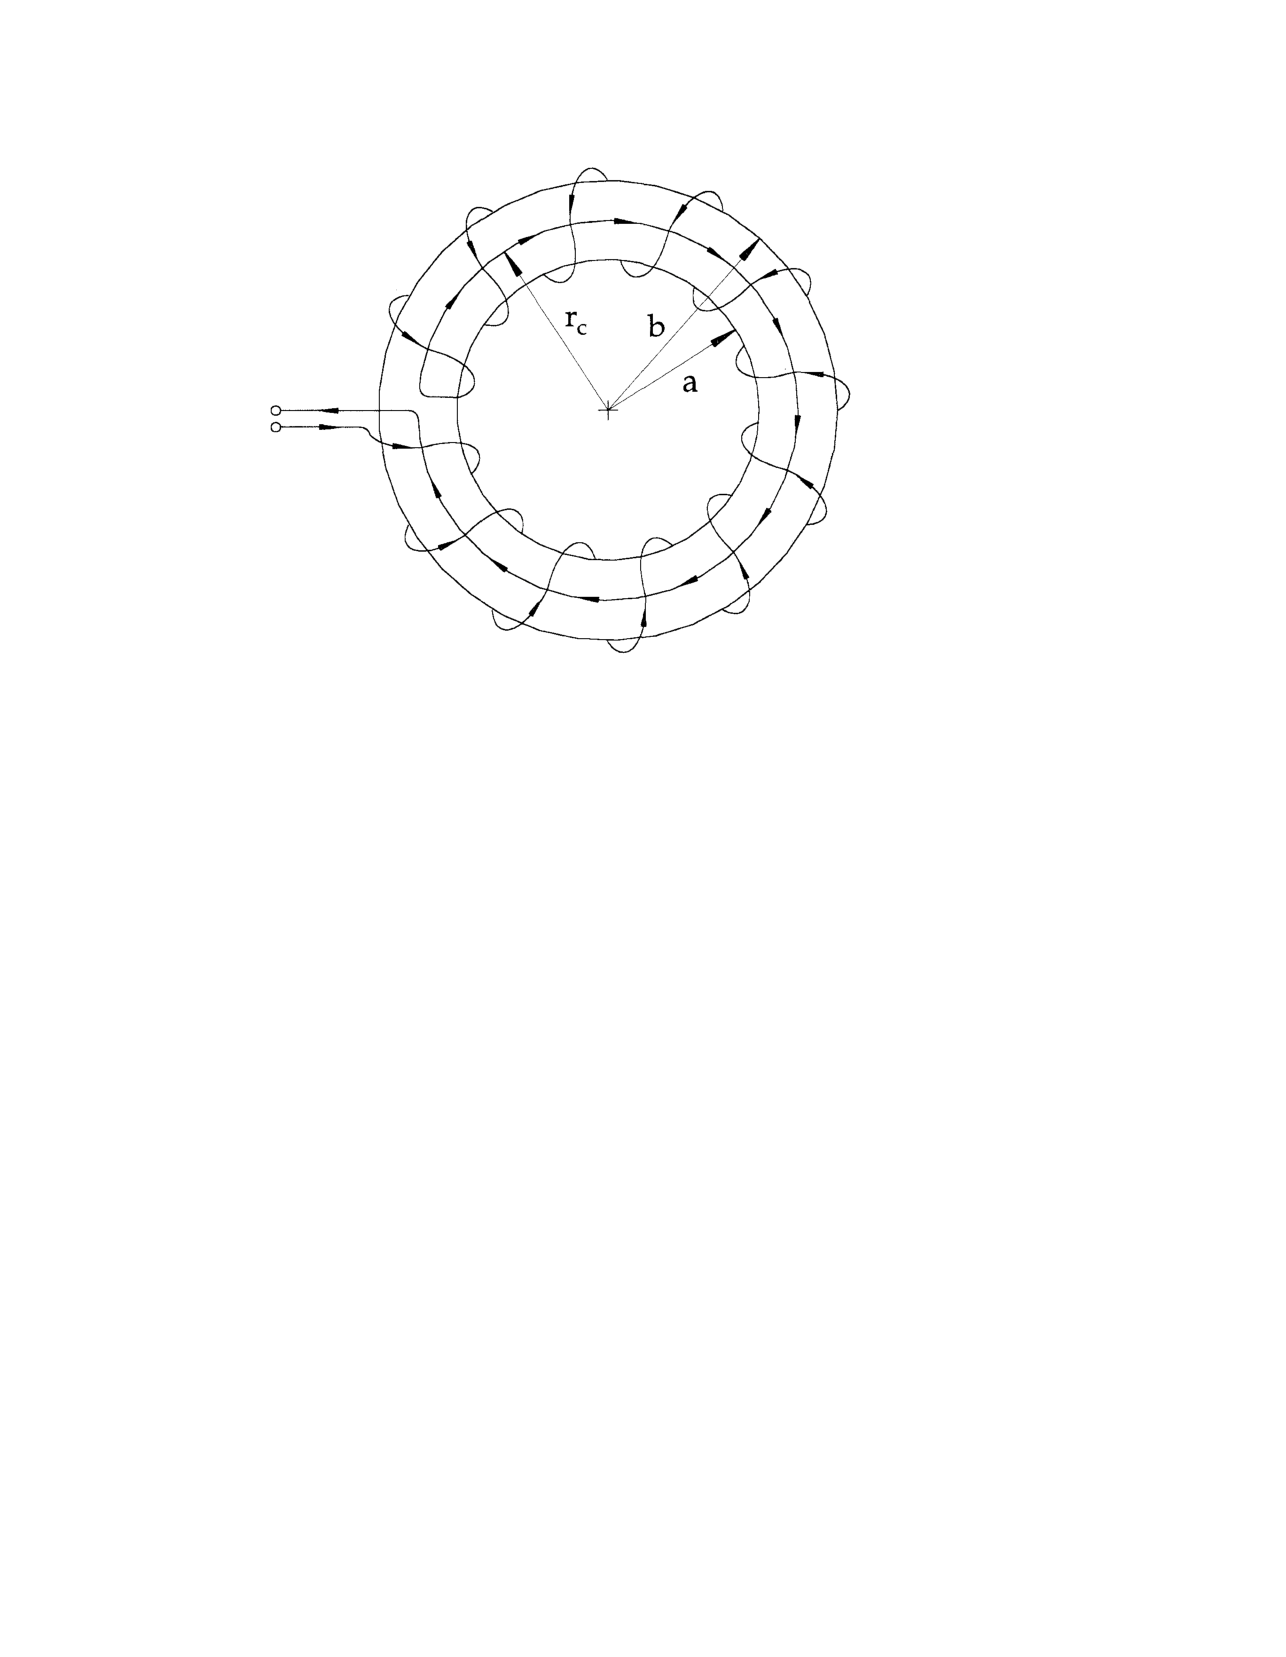
\includegraphics[width=0.5\textwidth]{rogowski.pdf}% Images in 100% size
  \caption{Single-layer Rogowski coil with a counter-wound compensation turn. The arrows indicate the direction of winding. \citep{492777}}
\label{fig:rogowski}
\end{figure}

\section{Electrostatic Diagnostics}

\subsection{Langmuir Probes}

An electrically biased conducting probe inserted into a steady-state plasma is known as a Langmuir probe, and is a surprisingly useful diagnostic tool particularly in low temperature plasmas. A probe larger than the Debye length is inherently perturbative and will draw current from the plasma. It is the perturbative nature of the probe which allows its use as a diagnostic tool, while simultaneously involving intricate interactions which require careful treatment in order to extract accurate the plasma density, electron temperature, and plasma potential. In this summary we will limit ourselves to the most straightforward case, that of a quasi-static, thermal, unmagnetized, relatively cold plasma.

Consider a probe which is biased at $V_p$ (with respect to the walls of the walls of the plasma chamber) is swept over a wide range, we measure the current flowing through the probe and obtain an I-V characteristic similar to that shown in Figure \ref{fig:langmuir}. At point B when the probe is at the floating potential $V_f$, the total current flowing out of the probe is zero. As the potential is decreased, eventually all of the electrons are repelled (point A) and the current approaches the ion saturation current $I_{is}$. Increasing the voltage from $V_f$, there is a distinct ``knee'' in the I-V characteristic at point C. This is the plasma potential (or space potential) $V_{sp}$ which is greater than $V_f$ due to the perturbative effect of the probe. The current at point C is the electron saturation current $I_{es}$. In the absence of collisions and sheath effects, the current would not increase for $V_p > V_{sp}$ since all electrons reaching the probe are collected and all ions are repelled.
\begin{figure}
  \centering
  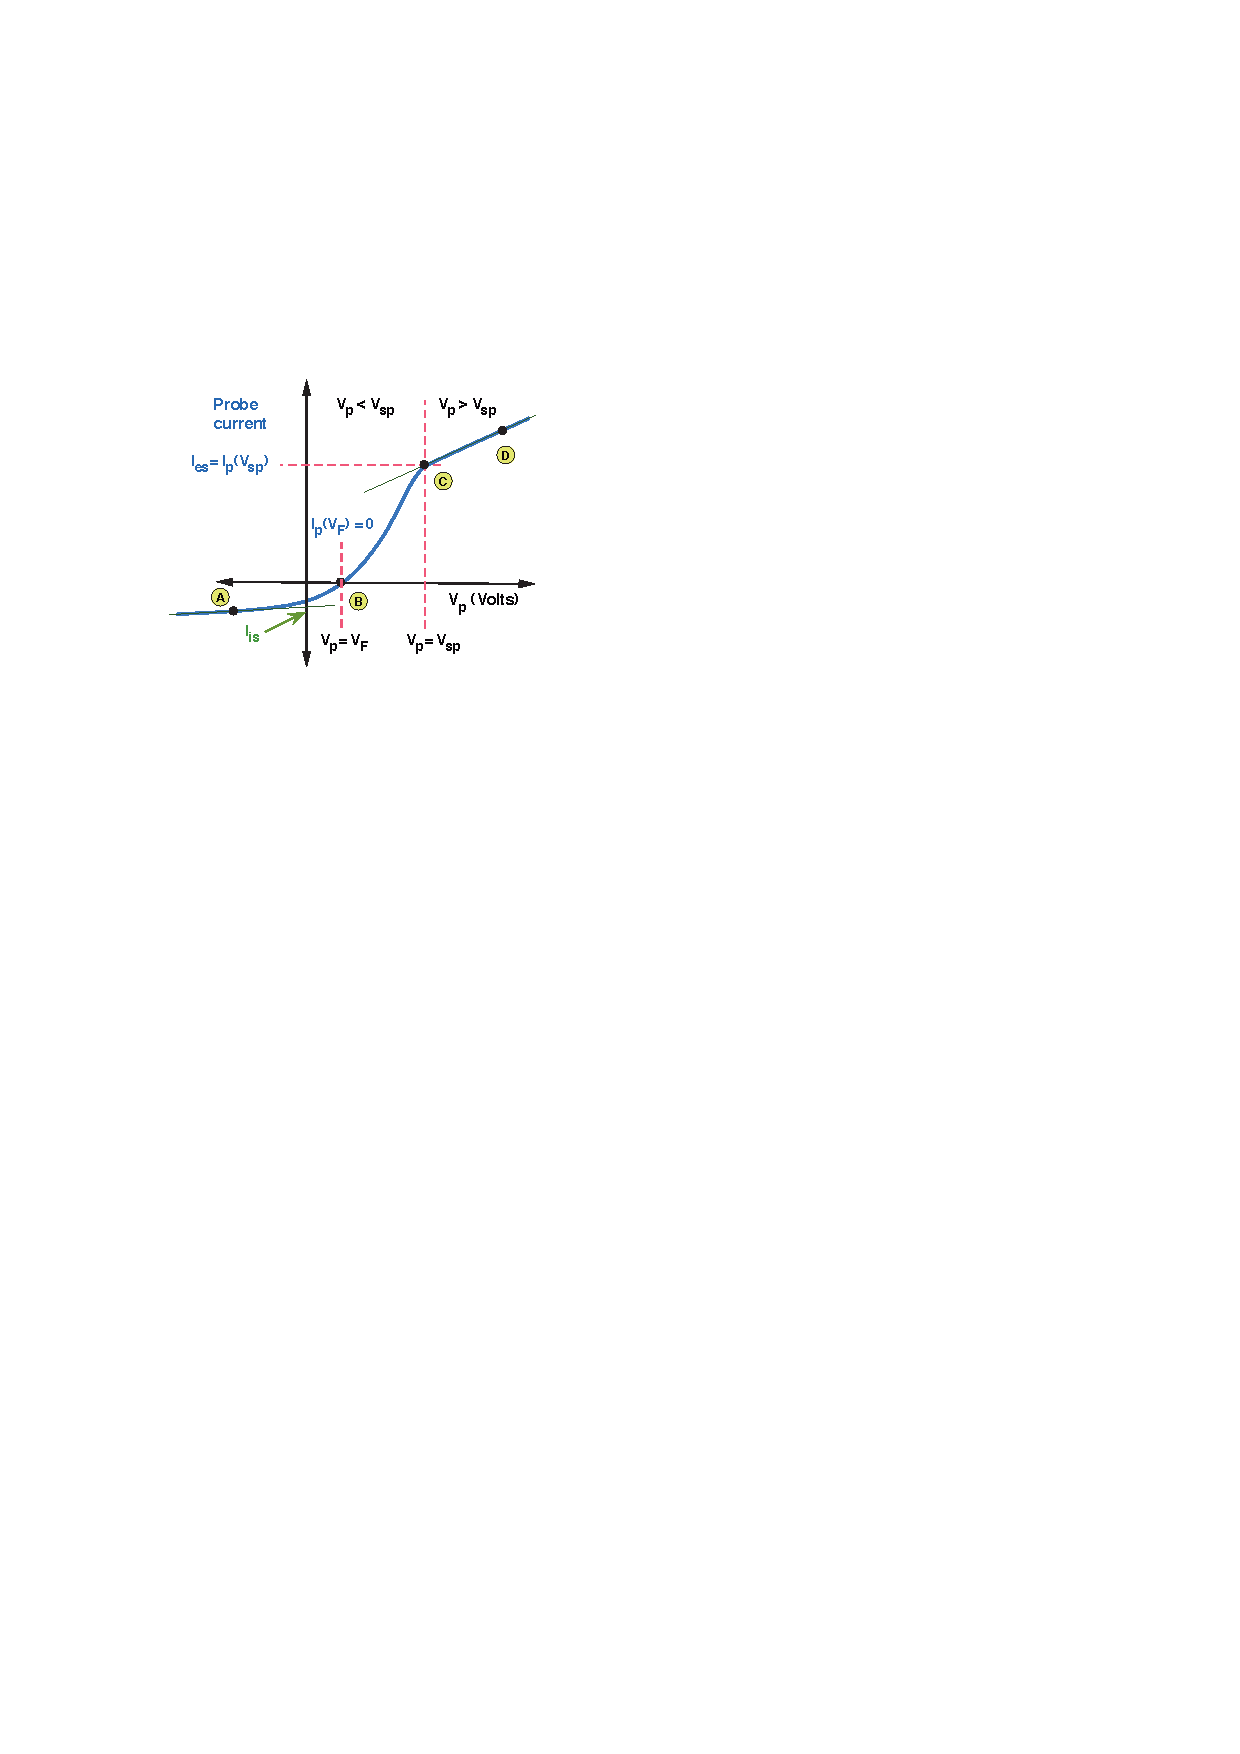
\includegraphics[width=0.5\textwidth]{langmuir-iv-curve.pdf}
  \caption{An idealized IV curve obtained with a collecting Langmuir probe in a cold plasma. \citep{Conde2011AnIT}.}
\label{fig:langmuir}
\end{figure}
The region between points B and C is called the transition region and is the region of interest in determining plasma properties. In the transition region, the electron current varies exponentially as $I_e = I_{es} \exp [(V_p - V_{sp})/ k T_e]$. Plotting $\ln(I)$ vs $V_p$, the slope of the transition region gives the inverse of the electron temperature $T_e$. With the temperature in hand, the plasma density can be determined from either the ion or electron saturation current:
\begin{equation*}
n_e = \frac{I_{is}}{e A} \left( \frac{m_i}{m_e} \right)^{1/2} \left( \frac{k T_e}{2 \pi m_e} \right) ^{1/2}
\end{equation*}
where $A$ is the probe area, $m_i$ is the ion mass, $m_e$ is the electron mass. Because the electron saturation current can be exceedingly large, the ion saturation current is much easier to determine. The presence of non-thermal energetic populations will create additional inflection points in the I-V characteristic.

Fluctuations in the plasma potential can push a single Langmuir probe into the electron saturation region, damaging or destroying the probe. A double Langmuir solves this problem by replacing the probe ground with a second floating probe of the same geometry and collection area, so that the probe current is based on the bias potential instead of the plasma potential with respect to the chamber wall. If the plasma parameters vary rapidly, the quasi-static assumption limits the time resolution of the measurement. Adding a third probe allows simultaneous measurement of multiple points along the I-V characteristic \citep{doi:10.1063/1.1714492}. To achieve simultaneous measurement of $T_e$ and $n_e$, we apply a large bias voltage between the first two probes to measure the ion saturation current as we would for a double probe. If set the voltage between probes 2 and 3 $V_{2,3}$ less than the difference between the floating potential and the plasma potential, the third probe operates in the transition region where $I_e = I_{es} \exp [(V_p - V_{sp})/ k T_e]$. The current through the double probe, the bias voltage, and $V_{2, 3}$ are then sufficient to simultaneously solve the current through each probe and recover an instantaneous measurement of $T_e$ and $n_i$.


\subsection{Gridded Energy Analyzers}

Langmuir probes can be used to obtain direct measurements of the electron temperature, but the electron saturation current is large enough to drown out any variations in the ion current. Instead, we can obtain a direct measurement of the ion energy distribution function by passing the ions through a system of grids at different potentials. A gridded energy analyzer is composed of a series of three wire grids maintained at various potentials and a charge collector. The first grid is held at a large negative potential to repel all incident electrons. The ions being positively charged pass directly through the first grid. A second grid is held at a positive grid potential $V_g$ and acts as a discriminator for high energy ions. Any ions with energy less than $e V_g$ are repelled, and the rest pass through to a collector plate. By varying $V_g$ and measuring the collector plate current, we obtain a cumulative distribution function for the ion energy.

When high energy ions strike the collector, they have a chance to liberate electrons which can escape backwards through the ion repeller. This has the effect of artificially increasing the measured collector current, obscuring the relatively weak signal at the upper tail of the ion velocity distribution. To avoid this situation, a third grid is placed between the ion repeller and the collector and maintained at a large negative potential, preventing electron escape from the collector. This configuration has the added benefit of separating the repellers from the collector, preventing stray currents within the repeller grids from affecting the measured collector current.

If the Debye length is small compared to the grid spacing, Debye shielding will reduce the effect of the grid fields. In high density plasmas where the Debye length can be a fraction of a millimeter, achieving such a close grid spacing can be unrealistic. The Debye length can be increased by placing a plasma density filter at the entrance to the gridded energy analyzer. In practice this adds uncertainty to the effective area of the collector, but does not have a significant effect on the measured energy distribution.

\section{Self-emission from Bound Electrons}

\subsection{Charge Exchange Recombination Spectroscopy (CHERS)}

Line radiation from partially-ionized low-Z impurity atoms in the plasma can be an effective method of determining the ion temperature. In large, very hot, dense plasmas, low-Z impurities in the plasma are completely ionized and do not emit line radiation. The presence of heavy high-Z ions for the purpose of photon measurements can have undesirable effects on the total heating requirements and radiation loss of the plasma. These limitations can be resolved by introducing a source of fast neutral atoms and measuring the line profiles of transitions excited by charge-exchange recombination reactions \citep{doi:10.1063/1.93893}, a diagnostic now known as CHarge Exchange Recombination Spectroscopy (CHERS). Many large-scale plasma experiments already feature a neutral beam injector for heating, doping, or diagnostic purposes which is suitable for CHERS measurements.

When collisions occur between fully-ionized light impurities in the plasma and a fast neutral beam of hydrogen atoms, a charge transfer can occur with a large cross-section:
\begin{equation*}
H^0 + A^{+Z} \rightarrow H^+ + A^{+Z - 1}
\end{equation*}
producing an excited hydrogen-like atom which quickly decays, emitting line radiation which can be analyzed for Doppler broadening and shifts. The radiating transition must cascade downwards in a series of angular momentum conserving transitions, with the result that the observed radiation will have a long wavelength. In high-energy experiments in which injection of impurities may be undesirable, injecting a neutral beam of the same species as the plasma ion species prevents contamination. The heavy ion loses very little momentum through the collision, such that the broadening of the resulting line radiation is representative of the temperature and velocity of the CHERS-ing ions.

The spectral information obtained via CHERS is inherently chord-integrated. Aligning the observation line of sight orthogonal to the beam path localizes the measurement, but there are several major sources of radiation that can coincide with the charge recombination line radiation. Bremsstrahlung broadband radiation, possible coincident lines with unrelated radiative transitions very close to the CHERS transition of interest, and the low-temperature tail of ions that have not been fully stripped will all contribute to the chord-integrated measurement. Modulation of the neutral beam can aid in distinguishing signal from background and reducing these errors.


\subsection{Laser-Induced Fluorescence (LIF) and Two-photon Absorption LIF (TALIF)}

Self-emission of bound electrons can be actively stimulated by inducing excitations with electromagnetic radiation at a resonant frequency, generally using a laser. Analysis of the resulting laser-induced fluorescence (LIF) has several advantages over passive spectroscopy. The intensity of line radiation for a particular transition can be increased substantially by tuning the laser frequency to the resonant frequency of the transition, and crossing the viewing and exciting beams can spatially localize what would otherwise be a chord-integrated measurement as shown in Figure \ref{fig:lif}. The effect of laser-induced excitations on the plasma properties is minimized by using a low-intensity beam or by pulsing the laser quickly to ensure that the target species only remains in an excited state for a very short amount of time (typically $\sim 10ns$). LIF is widely used in many fields outside of fusion plasma diagnostics. Within the scope of fusion plasmas, the spectra of the resulting radiation can provide information about ion temperature, density, and bulk velocity, and isotopic distribution.
\begin{figure}
  \centering
  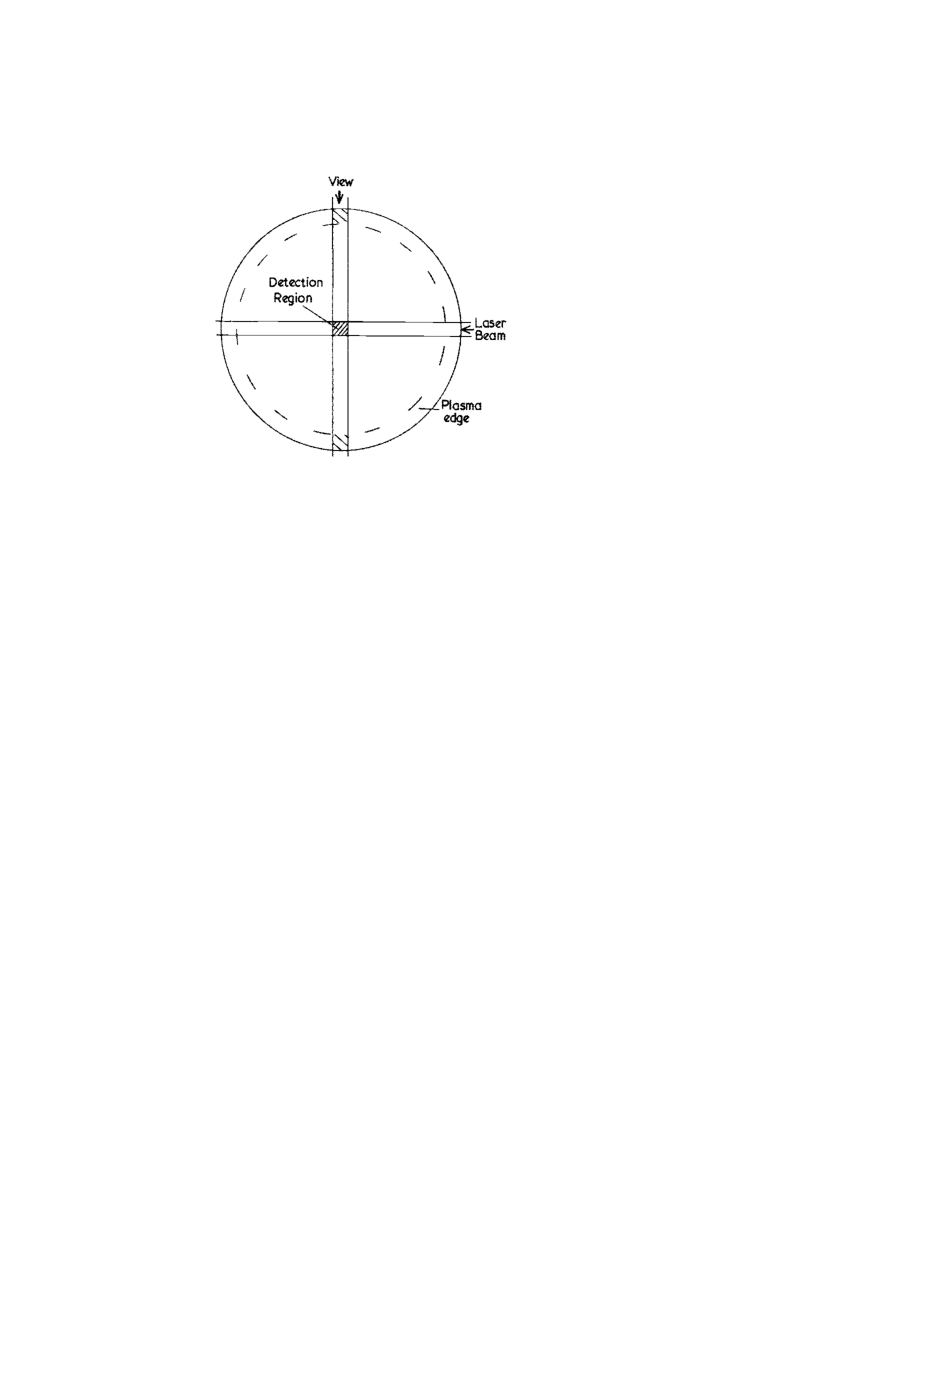
\includegraphics[width=0.5\textwidth]{lif-localized-region.pdf}
  \caption{Resonant fluorescence of atomic transitions with orthogonal viewing direction allows a very localized detection region. \citep{Hutchinson_2002}.}
\label{fig:lif}
\end{figure}
In fusion plasma experiments using hydrogen isotopes, it is desirable to measure the properties of hydrogen neutrals near the plasma edge. The wavelengths of interest (i.e. hydrogen $L_\beta$ transitions) are in the ultraviolet range and are not easily transmitted through viewing port windows, making direct spectroscopic measurements of transitions to the ground state difficult. The recent commercial availability of reliable high-energy, high-intensity, narrow linewidth lasers allows for excitation via a two-photon absorption process known as TALIF \citep{MageeRM2012Atpa}. As each photon only needs to provide half of the transition energy, lasers of longer wavelengths can be used which are much easier to produce and transmit. While the single-photon absorption rate is proportional to the laser intensity, the two-photon absorption rate is proportional to the square of the intensity, so measurements can be spatially localized without the need for a perpendicular viewing chord by focusing the beam at the position of interest with a lens.

The absorbed photons can come from a single beam, or from multiple coincident beams. Counter-propagating beams can be used to obtain ``Doppler-free'' measurements. By tuning the energy of each beam such that they sum to the transition energy, the Doppler shifts of the absorbed photons are equal and opposite and cancel. Such a counter-propagating setup effectively probes the entire Doppler-broadened line without the need to scan the laser frequency. Doppler-free measurements remove the temperature broadening from the absorption spectra, allowing for the observation of weaker broadening and wavelength shift effects such as Zeeman and Stark broadening.

\subsection{Zeeman Spectroscopy}

Zeeman spectroscopy is a non-perturbative magnetic field diagnostic based on the splitting of emission or absorption lines due to the Zeeman effect. Using this method it is possible to obtain locally resolved magnetic field measurements within the plasma volume where material probes are not an option. Since magnetic field strength is tied to the current density distribution and determines resistivity, plasma dynamics, and energy balance, spatially resolved magnetic field diagnostics are of particular importance in the realm of fusion confinement. As the diagnostic method of focus in this summary, we will go into significantly more detail on the method and its applications.

\subsubsection{The Zeeman Effect}

The Zeeman effect is the splitting of the energy states of bound electrons in the presence of an externally applied magnetic field. It is a result of the magnetic dipole interaction between the external field and the electron's spin $\vec S$ and orbital angular momentum $L$:
\begin{equation*}
H_{Zeeman} = \frac{e}{2 m_e c} (\vec L + 2 \vec S) \cdot \vec B
\end{equation*}
Perturbation theory is required to determine the new energy states of the electron. If the strength of the external magnetic field is small compared to the spin-orbit coupling fine-structure term ($B < 10 T$ for laboratory plasmas of small atomic number), then we can simply compute the expectation values of $H_{Zeeman}$ and add them to the energy states of the electron in the absence of the field. This is the ``weak'' Zeeman effect; for very strong magnetic fields the spin-orbit coupling is broken and the effect is known as the Paschen-Back effect. For a weak magnetic field, we assume without loss of generality that the magnetic field points in the z-direction and compute the energy splitting $E_{Zeeman}$ as
\begin{equation*}
E_{Zeeman} = g_J \mu_B m_j B
\end{equation*}
where $g_J$ is the Landé g-factor (which depends on the quantum numbers $j$, $l$, and $s$), $m_j$ is the z-component of the total angular momentum, and $\mu_B$ is the Bohr magneton. In an absorption/emission spectrum, this translates to a wavelength shift $\Delta \lambda$ given by:
\begin{equation*}
\Delta \lambda = \frac{\mu_B}{h c} \Delta (m_j g_J) B \lambda_0 ^2
\end{equation*}
An external magnetic field thus broadens a spectral line $\lambda _0$ by an amount proportional to the field strength, the wavelength of the line, and the difference $\Delta (m_j g_J)$ between the transition states.

\subsubsection{Broadening Effects}

\begin{figure}
  \centering
  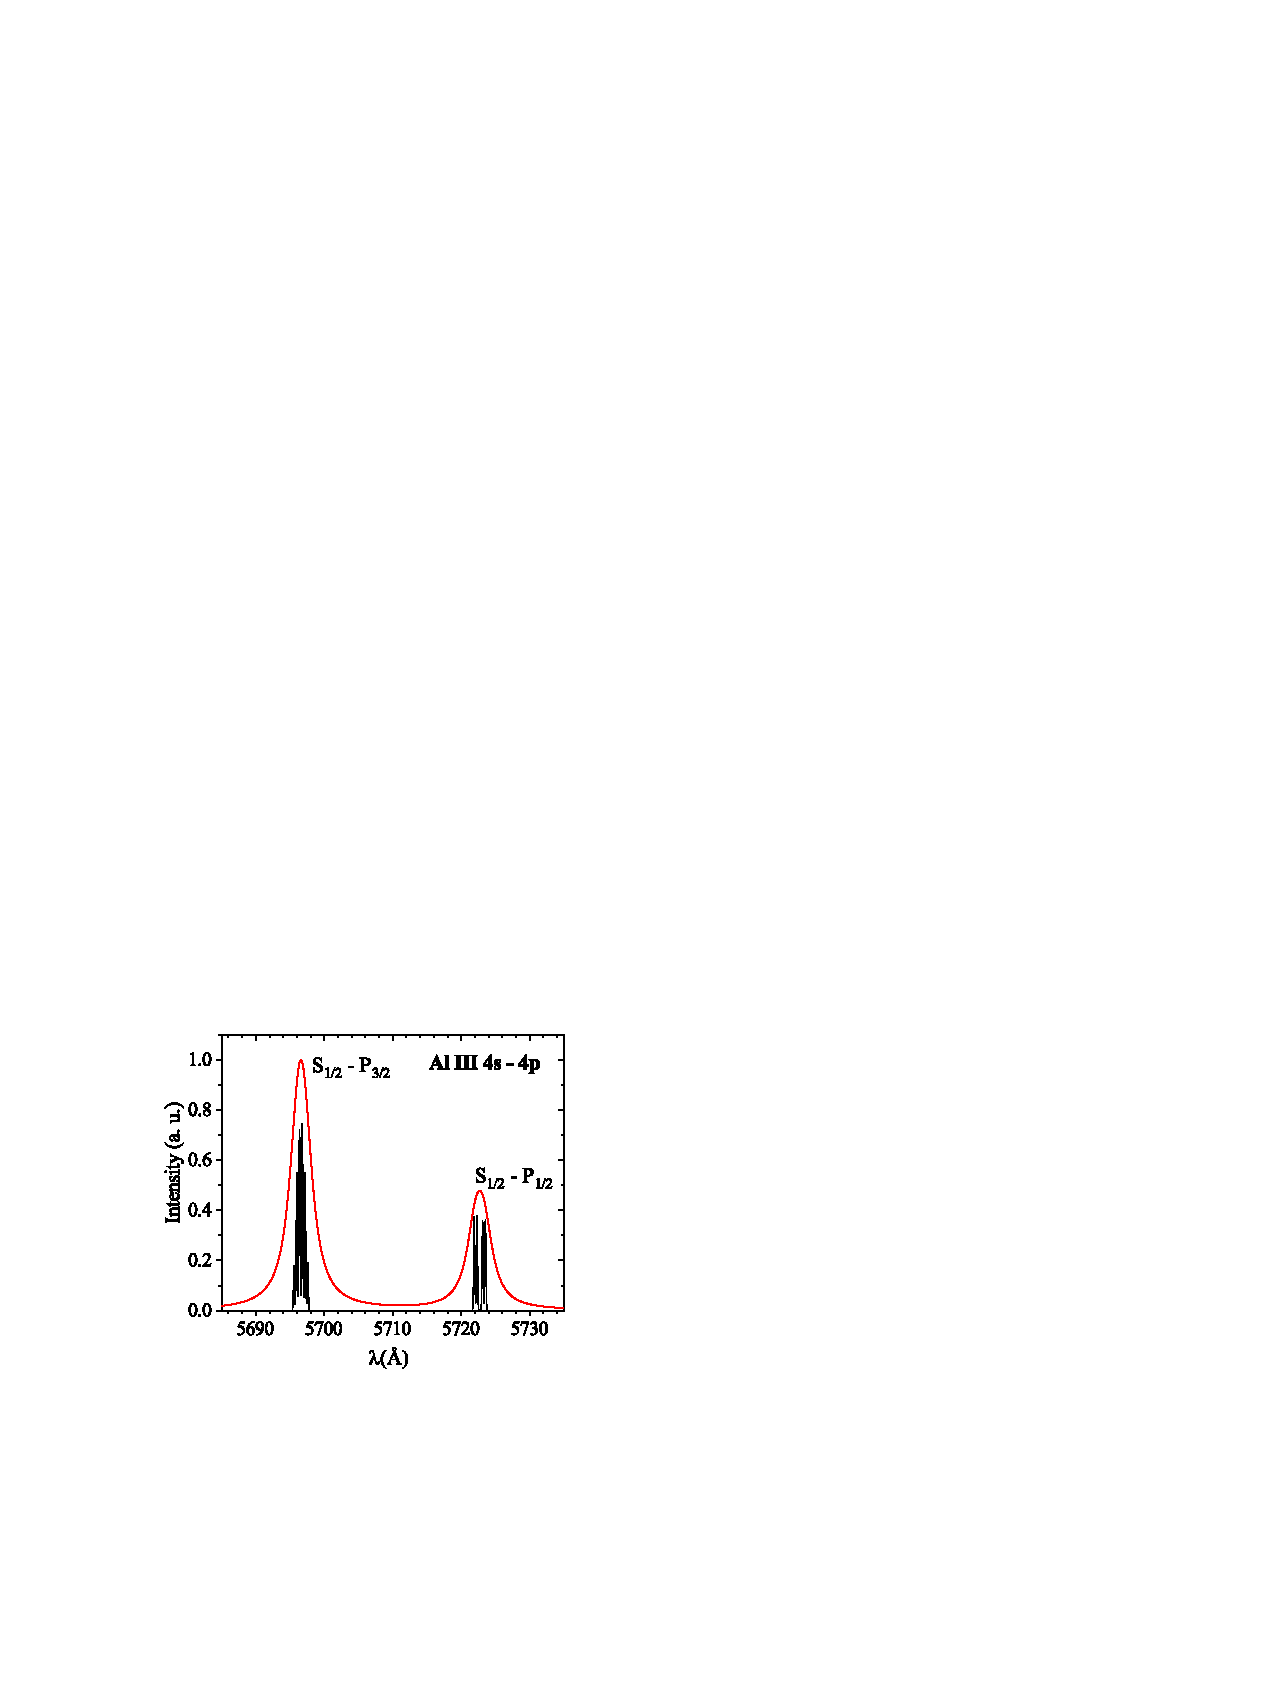
\includegraphics[width=0.6\textwidth]{pres7.pdf}
  \caption{Shown in red is Zeeman effect of the Al III 4s-4p doublet, calculated for a magnetic field of 4T and convolved with Voight profile due to a $0.2\angstrom$ FWHM Doppler-Gaussian ($T_i= 5 eV$) and a $3\angstrom$ Lorentzian ($n_e = 5 \cdot 10^{17} cm^{-3}$). Also shown in black is the Zeeman pattern without the Lorentzian broadening. From \citep{doi:10.1063/5.0009432}.}
\label{fig:broadening}
\end{figure}

The line splitting due to the Zeeman effect can be very small when compared with other sources of line broadening present in high energy density plasmas. In a high density $n_e = 10^{17} cm^{-3}$ plasma, the width of the Lorentzian pressure broadening can be an order of magnitude greater than the Zeeman splitting, as shown in Figure \ref{fig:broadening}. Likewise, the Gaussian temperature broadening in a fairly low-temperature plasma $T = 5 eV$ will be as large as the Zeeman splitting. Instrument broadening will contribute an additional broadening term. While the Zeeman splitting may be measured directly in relatively cool, thin plasmas, it can be very difficult to extend Zeeman splitting diagnostics to high energy density plasmas. Fortunately, it is possible to use polarization discrimination to discern the separate Zeeman split components even in the presence of substantial broadening.

\subsubsection{Polarization Effects}

Selection rules governing electric dipole transitions mandate that for a given transition $\Delta m_j = 0$ or $\Delta m_j = \pm 1$. Transitions for which $\Delta m = 0$ are called the $\pi$ components. The $\Delta m = \pm 1$ components are $\sigma^+$ and $\sigma _-$, respectively. The $\sigma$ components are split further from the original line since $\Delta (m_j g_J)$ is greater for $\Delta m = \pm 1$. Because the emitted/absorbed photon has unitary spin, conservation of angular momentum uniquely determines the polarization of each component, as shown in Figure \ref{fig:zeeman-polarization}. The $\pi$ component is linearly polarized parallel to the magnetic field. The $\sigma$ components are circularly polarized in the plane perpendicular to the magnetic field. This leads to two possible orthogonal viewing situations. When viewed along a line of sight parallel to the magnetic field, the un-shifted $\pi$ component is not observed and the $\sigma$ components are observed with opposite circular polarization. When viewed along a line of sight perpendicular to the magnetic field, the $\pi$ component is observed linearly polarized parallel to the magnetic field, and the $\sigma$ components are observed linearly polarized perpendicular to $\vec B$. Because the thermal and pressure broadening effects are polarization independent, polarization discrimination can be used to recover the otherwise obscured Zeeman broadening at high temperatures and pressures.

\begin{figure}
  \centering
  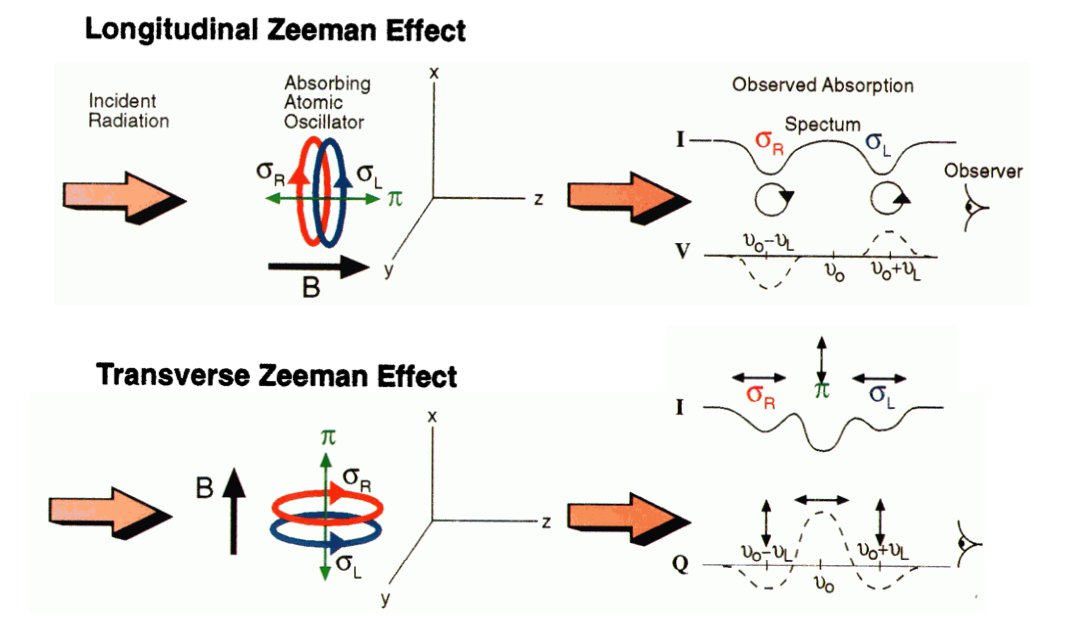
\includegraphics[width=0.7\textwidth]{pres4cropped.png}
  \caption{Depiction of the $\sigma$ and $\pi$ components of the Zeeman split transition when viewed longitudinally or transverse to the direction of the magnetic field. In the transverse view, the $\pi$ and $\sigma$ components are both visible and are linearly polarized orthogonal to each other. In the longitudinal view, the $\sigma$ components are right- and left-circular polarized and the $\pi$ component is no longer visible. \citep{https://doi.org/10.1029/1999RG900011}.}
\label{fig:zeeman-polarization}
\end{figure}

\subsubsection{Transverse Zeeman Diagnostic}

In a Z-pinch configuration, the magnetic field is completely azimuthal at all locations and the observational line of sight may be oriented parallel the z-axis so that it is perpendicular to the direction of the magnetic field. In this transverse view, both $\pi$ and $\sigma$ components will be visible with linear polarization as shown in Figure \ref{fig:zeeman-polarization}. Under the assumption that the plasma parameters are constant along the z-axis, this produces a measurement which is radially resolved. The $\pi$ and $\sigma$ components can be separated by their orthogonal linear polarization, but remain convolved with the other sources of broadening.

The Zeeman splitting is determined by calculating a fit of the broadened spectral line for each of the $\pi$ and $\sigma$ components using the full expression for the convolved Zeeman splitting and sources of broadening. The difference in FWHM between the components gives the Zeeman splitting, which in turn gives the magnetic field strength. Computing the field in this manner requires a very high signal-to-noise ratio, and is typically not possible to achieve in a single shot. The method is not appropriate for a configuration with low shot-to-shot reproducibility, but has the benefit of obtaining radially-resolved magnetic field measurements without the need for inversion.

\subsubsection{Longitudinal Zeeman Diagnostic (Two-Polarizations Method)}

In contrast, if the observational line of sight can be aligned parallel to the magnetic field, then the $\sigma^+$ and $\sigma ^-$ components can be separately identified by polarization. This gives the most sensitive possible measurement of the Zeeman splitting by suppressing the un-shifted $\pi$ components. However, in a Z-pinch configuration, the only observation chord which is strictly parallel to the magnetic field is a line tangent to the outermost radius of the plasma extent which only provides the magnitude of the field at a single radius. The ``two-polarizations method'' resolves this restriction by making use of the significant temperature gradient present in a Z-pinch, as shown in Figure \ref{fig:impurity-shells} using the example of oxygen impurities. At the cooler larger radii, the plasma is only hot enough to doubly ionize oxygen, so the oxygen population at that radius will be predominantly O-III. As the temperature increases towards the center of the pinch, the charge state of oxygen will continue to increase. The charges of O-III and O-VI are sufficiently different that they reside in distinctly different radii. The unique emission lines of the different charge states can be identified and analyzed for Zeeman splitting.

\begin{figure}
  \centering
  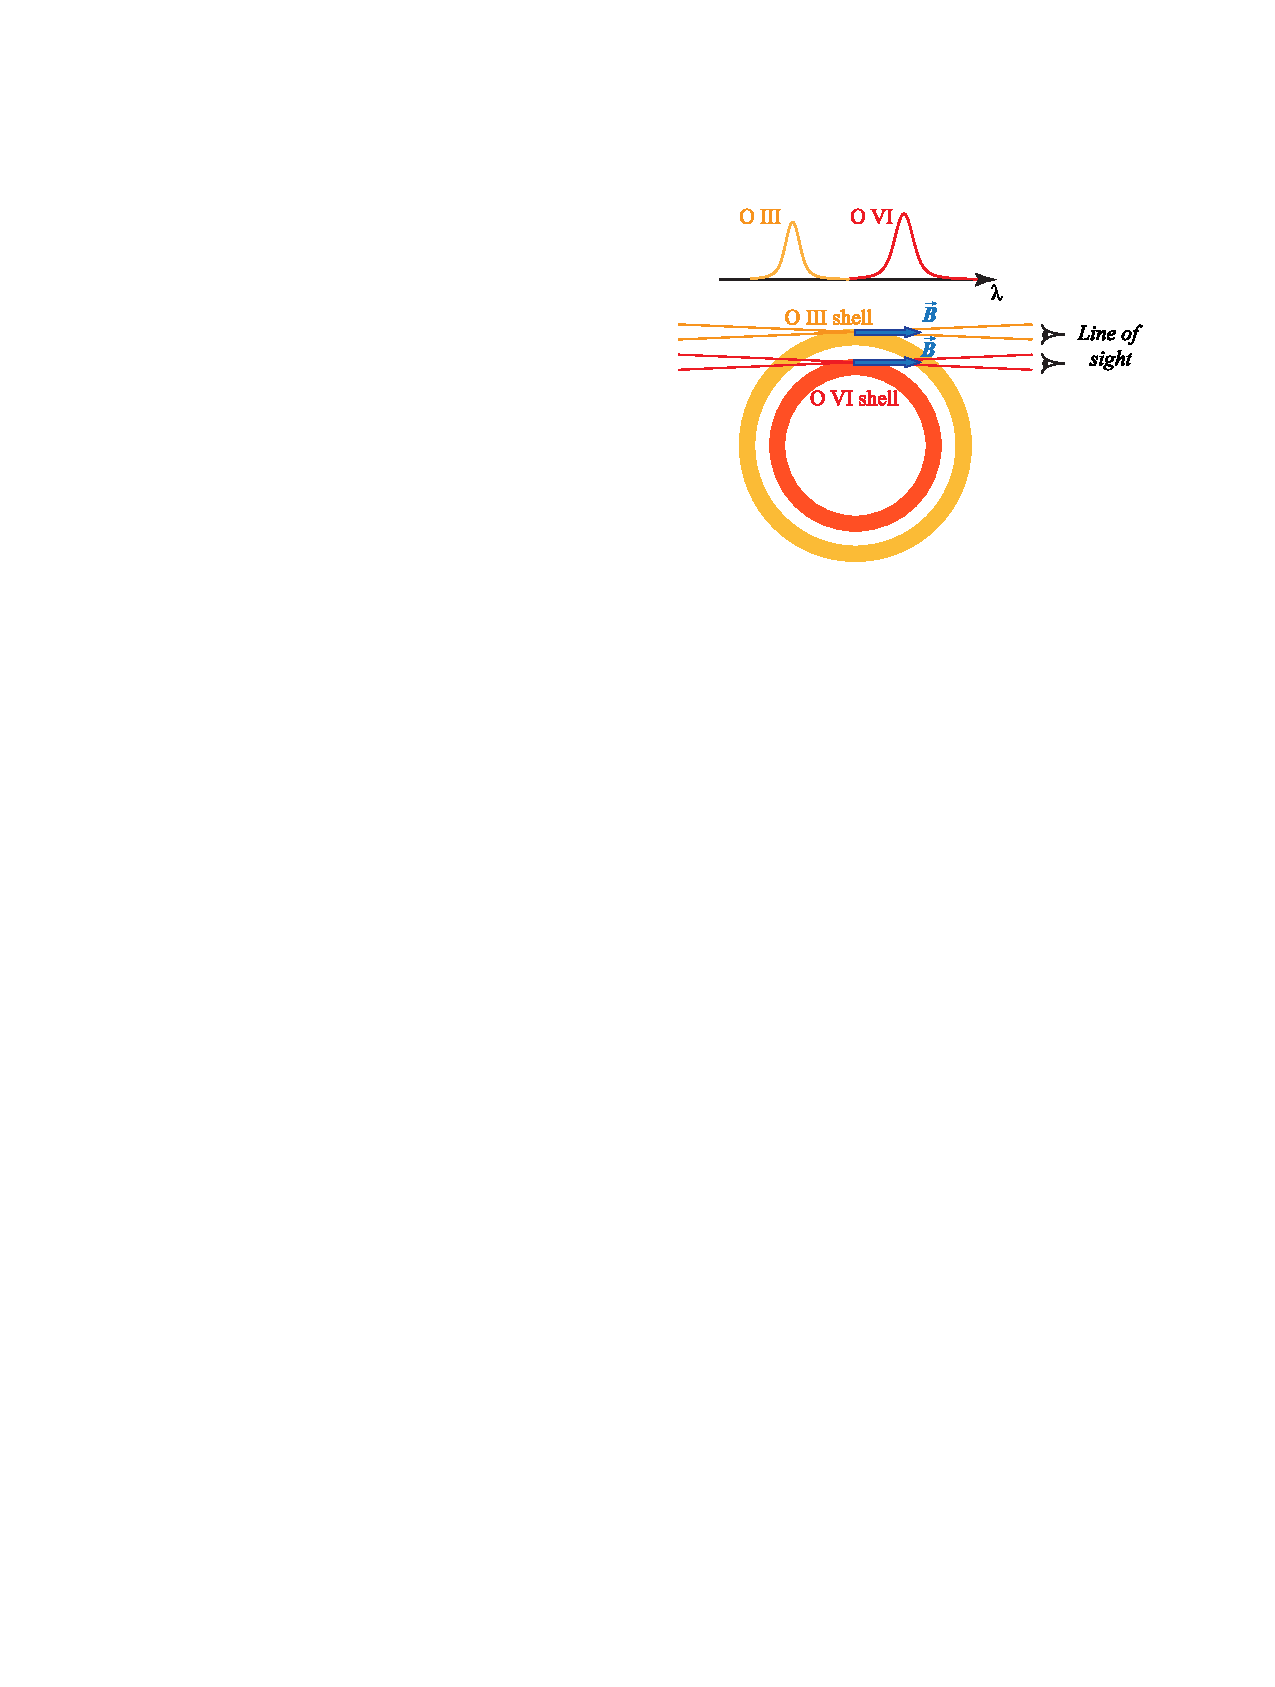
\includegraphics[width=0.7\textwidth]{impurity-shells.pdf}
  \caption{Schematic of measurements of the B-field radial distribution by utilizing the emission lines of different charge states that are abundant within different radii. Observing the emission from the outermost radius in which each charge-state emits provides radially resolved data without the need for Abel inversion. It also ensures viewing parallel to the magnetic field, which is crucial for polarization spectroscopy. From \citep{doi:10.1063/5.0009432}}
\label{fig:impurity-shells}
\end{figure}

In practice, the temperature distribution and distribution of charge state populations may not be known a priori. Instead, observations are made along many chordal lines of sight to identify the maximum radius in which the various charge states reside. At this radius, the magnetic field is nearly parallel to the line of sight as shown in Figure \ref{fig:impurity-shells}, and the un-shifted $\pi$ component is completely suppressed. The $\sigma^-$ and $\sigma^+$ components can then be separated by combining a quarter-wave plate and a beam splitter. The Zeeman splitting can then be calculated from the shift in line positions between the split components. Since this method relies on the line positions rather than their shapes, this has the highest sensitivity to the magnetic field and can be performed in a single measurement. This method was used to generate a distribution of the magnetic field strength at several times during a single pulse in a Z-pinch device by \citep{Rosenzweig_2017}. An additional data point of boundary field strength can be obtained from Ampère's law using a B-dot probe outside the pinch region, assuming the total current flows within the plasma cylinder.

This method can provide exceptionally detailed information about the magnetic field distribution compared to other methods without the need for Abel inversion. The predominant sources of error inherent to this method are the finite acceptance cones of the optical elements, the polarization mixing between branches in the quarter-wave plate for non-zero angles of incidence, the decrease in diattenuation of the polarizing beam splitter at angles of incidence other than $45^\circ$, and any components of the magnetic field which are not parallel to the line of sight. Each of these effects serves to decrease the observed splitting, making the derived magnetic field a lower bound for the true field. The technique is generally limited to a minimum radius from the pinch axis. Closer to the axis, the temperature is maximized (increasing Doppler broadening) and the field strength is minimized, decreasing the observed Zeeman splitting.

% \subsubsection{Measurements of Magnetic Field with Arbitrary Direction}

\subsubsection{Neutral Particle Injection}

Line radiation spectroscopic techniques require the presence of species within the plasma volume which have not been fully ionized. In high energy tokamaks, the presence of many high-Z impurities within the bulk plasma can cause unacceptable radiation losses and power requirements. Even in experiments with substantial intrinsic impurity populations, localized injection of neutral atoms can help localize the otherwise chord-integrated measurement. Neutral species for line radiation spectroscopy are typically injected using diagnostic neutral beam injectors or pellet injection.

Neutral beams are often present in large-scale fusion confinement experiments to perform a variety of diagnostics. A high-energy beam of neutral atoms is injected into the plasma where it becomes excited by collisions with the plasma and emits Zeeman-split line radiation. Lithium neutral beams have been used for Zeeman spectroscopy on the DIII-D experiment \citep{doi:10.1063/1.1526928} due to the long wavelength of the $2^2S$-$2^2P$ transition and the minimally perturbative effect. Intersecting the line of observation with the neutral beam in a small volume gives a localized measurement of the field strength. With a highly-localized measurement, the direction of an unknown magnetic field can be determined by calculation of the ratio of linear to circular polarization. For Zeeman spectroscopy of an injected neutral beam to be successful, the beam must be generated with extremely low intrinsic ion temperatures to reduce the Doppler broadening as much as possible. The beam current must strike a balance; higher beam current produces a better signal-to-noise ratio, but can push the diagnostic into a perturbative regime by injecting a large impurity population.

Pellet injection is also used in high-energy experiments to introduce localized impurity species. Pellet injectors are frequently used to refuel the burning plasma or to trigger stabilizing edge localized modes \citep{BaylorL.R2015Emwp}. Small pellets are injected at high speed into the plasma where they vaporize, forming a roughly localized ablation cloud. Line radiation from the ablation cloud can then be analyzed for Zeeman splitting measurements. This technique is used in the Tokamak Fusion Test Reactor \citep{doi:10.1063/1.1141775} using lithium pellet injection to determine the magnetic field direction.

\section{Thomson Scattering}

Thomson scattering is the elastic scattering of electromagnetic radiation from free charged particles in the classical limit. Although the Thomson scattering cross section is extremely small, laser sources of sufficient power ($>100 MW$) to observe Thomson scattering above the background radiation have become commercially available and Thomson scattering measurements have become commonplace in both magnetic fusion and inertial confinement fusion research \citep{doi:10.1063/1.2336451}. Two distinct categories of Thomson scattering measurements can be identified by the product of the wavevector of the scattered radiation and the Debye wavelength. For $k \lambda_{De} \gg 1$, the electrons scatter independently and the scattering is incoherent. When the wavelength is larger than the Debye length, resonant plasma fluctuations form collective effects and the scattering is coherent.

\subsection{Incoherent Thomson Scattering}

Thomson scattering from electrons is ``incoherent'' when the Debye length is much greater than the wavelength of the scattering laser such that the collective plasma effects can be neglected in the scattering interaction. The spectrum and intensity of the scattered light can be used to determine the density and temperature of electrons. This has major advantages over other methods of electron temperature measurement. Langmuir probes perturb the plasma and are limited to the plasma edge. Interferometry gives chord-integrated measurements which must be inverted to spatially resolve. In contrast, coherent Thomson scattering is a direct, localized, weakly-perturbing diagnostic.

An incoherent Thomson scattering setup involves a pulsed laser source, an optical collection system with an observation line intersecting the laser path, and a spectrometer capable of resolving narrow wavelength separations. The wavelength of scattered radiation will be Doppler shifted by the thermal motion of the scattering electron, and the intensity of the scattered radiation is proportional to the number of scattering electrons in the scattering volume. Assuming a Maxwellian thermal distribution of electrons, fitting a Gaussian to the scattered radiation spectrum gives the electron temperature. If the spectrometer is capable of sufficiently detailed resolution in frequency space, the spectrum can also be analyzed for non-Maxwellian populations. Recovering the electron density from the scattered intensity requires an absolute calibration of the diagnostic using a neutral gas.

The scattering interaction cross-section for electrons is very small, determined by the total Thomson cross section $\sigma_t = 8 \pi r_e ^2 / 3 \approx 6.65\cdot 10^{-29} m^2$. Very high intensity laser sources are required to achieve acceptable signal-to-noise ratios. Laser sources in use are typically in the optical range, commonly ruby or frequency-doubled Nd:YAG lasers. The most prominent sources of noise are external sources, stray laser radiation, stray line radiation, and bremsstrahlung. During Thomson scattering measurements, noise from external sources is reduced by blocking sight-lines, covering windows, and using a viewing dump for the observational line. Stray laser radiation can be removed by blocking light within the laser bandwidth at the spectrometer. Coincident line radiation can be avoided by adjusting the laser frequency if using a dye laser or other tunable laser source. Bremsstrahlung is broad-band radiation which can not be spectrally filtered. Noise from bremsstrahlung can be reduced by shuttering the detector very quickly in tandem with the laser pulse. Polarized laser sources can also be used to further increase the signal-to-noise ratio.

The spectral and spatial resolution of Thomson scattering can be improved with more complicated configurations. In TV Thomson scattering, scattered radiation is collected using a group of lenses focused at multiple locations along the laser beam and imaged by position onto the detector slit. Light from the detector slit is then dispersed to form a 2D spectrogram along a spatial dimension. The optical configuration for such a detector can be very complicated, but the increased resolution can be worth the trouble. Incoherent Thomson scattering can also be performed using a single port by measuring backscattered radiation in a LIDAR configuration. Measurements are spatially resolved by the time of flight; backscattered radiation from points further from the detector will arrive later. The spatial resolution in LIDAR systems is largely determined by the laser pulse duration, and sub-nanosecond pulse durations are not uncommon. The maximum achievable pulse intensity and small Thomson scattering cross-section limit the achievable spatial resolution. As with pulsed polarimetry diagnostics, the commercial availability of high-intensity chirped pulse amplification sources has dramatically improved the spatial resolution that can be achieved.

\subsection{Coherent Thomson Scattering}

Coherent Thomson scattering occurs when the scattering wavelength covers multiple Debye lengths and resonant plasma fluctuations are observed. In this regime, the collective plasma effects can be observed to discern ion  temperature and density information as well as electron temperature. Rather than considering the scattering from an individual electron, the coherent effect must be computed as an integral over many electrons in a finite volume. The full calculation of the scattered power spectrum for a monoenergetic source is given in \citep{https://doi.org/10.1029/JZ065i009p02635}, and can be used to fit the observed scattered spectrum to accurately determine the electron temperature and density. The Thomson-scattered power is proportional to $1 - \sin ^2 \theta \cos ^2 \beta$, where $\theta$ is the angle between the laser and collection optics and $\beta$ is the angle of incident polarization relative to the scattering plane. Observation at an angle of $90^\circ$ with respect to the laser path gives the highest signal intensity, as does polarization of the laser within the scattering plane. Because $k \lambda_{De}$ decreases with decreased angle of incidence, forward scattering may be preferred to reach the coherent regime in low density plasmas where a sufficiently long laser wavelength is not feasible.

While we only observe scattering Thomson scattering from the electrons, because the plasma fluctuations occur over many particles the oscillations will also contain elusive information about the properties of the ions. As long as $Z T_e / T_i > k^2 \lambda _{De} ^2$, collective ion-acoustic features can be observed in the form of two  counter-propagating ion-acoustic waves. The wavelength separation between the ion-acoustic features is approximately
\begin{equation*}
\frac{\Delta \lambda}{\lambda_0} = \frac{4}{c} \sin \left( \frac{\theta}{2} \right) \sqrt{ \frac{ k_b T_e}{m_i} \left[ \frac{Z}{(1 + k ^2 \lambda_{De} ^2)} + \frac{3 T_i}{T_e}\right]}
\end{equation*}
where $m_i$ is the ion mass, $T_i$ is the ion temperature, $T_e$ is the electron temperature, and $Z$ is the ion charge. This is one of the few available direct measurements of the ion temperature. The ion bulk velocity can also be determined by measuring the Doppler shift in these features. In practice, impurities present in the plasma will tend to distort the observed spectrum, making accurate, unambiguous determination of the ion temperature challenging. Even so, the technique is currently in use to measure the ion temperature and velocity in tokamak experiments (ASDEX) and Hall thruster diagnostics (PRAXIS).

\section{VISAR}

A ``Velocity Interferometer System for Any Reflector'' (VISAR) is a diagnostic tool for measuring the velocity of fast-moving surfaces, often used to measure shock propagation in inertial confinement fusion research. As a velocity interferometry system, it computes the phase shift of light reflected from a fast-moving surface, which in turn is used to determine the velocity of the surface. Unlike most velocity interferometry measurements, VISAR is effective for diffuse, un-coated surfaces. The conventional VISAR system (shown in Figure \ref{fig:visar}) is comprised of a pair of wide-angle Michelson interferometers operating on different polarizations of light reflected from the moving surface. A wave plate in one leg of the interferometer adds a $90^\circ$ phase shift between the two polarizations. A third detector monitors the raw intensity of the input light.
\begin{figure}
  \centering
  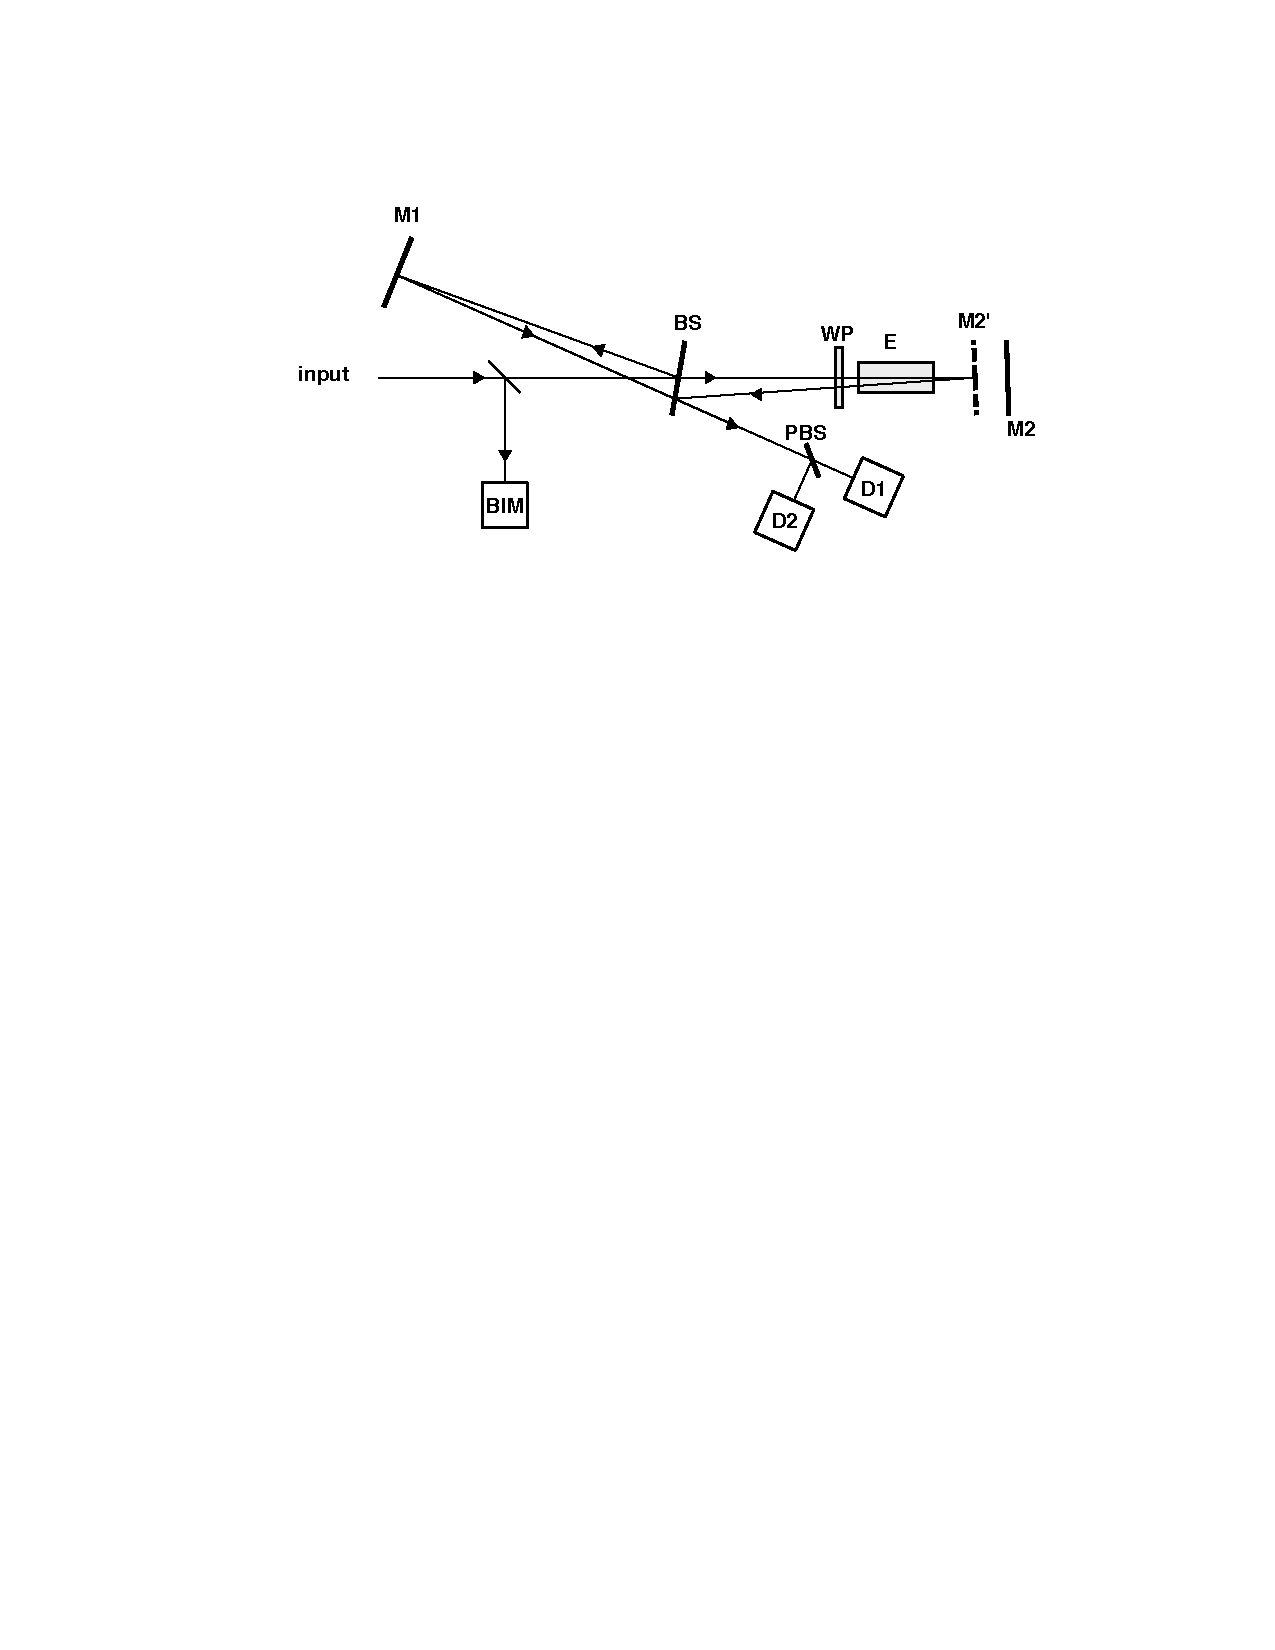
\includegraphics[width=0.6\textwidth]{visar.pdf}
  \caption{Diagram of the conventional VISAR setup, showing beam intensity monitor (BIM), beam splitter (BS), 1/8 wave plate (WP), etalon (E), mirrors (M1, M2), polarizing beam splitter (PBS), and detectors (D1, D2). From \citep{10.2172/886901}.}
\label{fig:visar}
\end{figure}
In this configuration, the phase of the input light $\phi(t)$ can be computed by plotting the intensities measured at the detectors $D1$ and $D2$ normalized by the beam intensity monitor signal on an ellipse defined by:
\begin{equation*}
D_x \equiv \frac{D_1(t)}{D_{BIM} (t)} \qquad D_y \equiv \frac{D_2 (t)}{D_{BIM}(t)} \qquad \tan \phi (t) = \tan \epsilon + \frac{D_y (t) - y_0 }{D_x (t) - x_0} A \sec \epsilon
\end{equation*}
where $x_0$, $y_0$, $A$, and $\epsilon$ are independent of the input power. Because the interferometer signal is normalized by the beam intensity monitor, the setup is insensitive to variations of the input intensity. This is what allows for velocity measurements of diffuse surfaces. The expression for $\tan \phi$ (in contrast to $\cos \phi$ for a single Michelson interferometer) makes it possible to remove the sign ambiguity from $\phi$ and distinguish velocities towards and away from the detector.

One drawback to the conventional VISAR setup is that only half of the incident light reaches the detectors, while the rest is lost to the opposite side of the beam splitter. We can add an additional VISAR on the other side of the beam splitter in place of the beam intensity monitor, generating a second set of signals very similar to the first pair. By pairwise subtracting the signals using electronic differential amplifiers (to impart a $180^\circ$ phase shift), the result is known as a push-pull VISAR. The phase of the input light can then be calculated from the resulting pair of signals in the same manner as a conventional VISAR. The additional light efficiency can improve the noise efficiency of the VISAR by approximately $40\%$ over a conventional VISAR, and if properly balanced is insensitive to variations in the input intensity and incoherent light \citep{10.2172/886901}. The push-pull VISAR has largely supplanted conventional VISAR in most applications.

\section{Pulsed Polarimetry}

A promising new magnetic field diagnostic is a LIDAR-like method known as fast-pulsed polarimetry. This method has the potential to resolve some of the most severe limitations of Faraday rotation measurements, providing spatially resolved measurements without the need for inversion of chord-integrated data. The technique combines standard Faraday rotation polarimetry \citep{Pisarczyk1990} and  with a pulsed ranging detection scheme in order to 

LIDAR (Light Detection and Ranging) has long been used to generate spatial profiles of distant objects by recording reflections from a pulsed laser source. Devices capable of high power chirped pulse amplification \citep{STRICKLAND1985219} are now available, opening the door to apply pulsed ranging schemes to dense energetic plasmas with millimeter spatial resolution.

{\Large TODO \par}

\section{Neutron Diagnostics}

In fusion research experiments, nuclear fusion reaction rates are of primary interest, both as a measure of the successful production of energy and as a diagnostic for the ions in the plasma. Nuclear reactions in deuterium and deuterium-tritium plasmas produce high-energy neutrons which, being uncharged, can escape the plasma to be registered by a diagnostic system. The intensity and spectra of these daughter neutrons contain valuable plasma diagnostic information. As the cross-section for the neutron-producing reactions are well known and strong functions of ion temperature, the daughter neutron flux can be used to estimate the temperature in a way that is insensitive to errors in the ion density \citep[p. 371]{Hutchinson_2002}. With measurements of spatial emission profiles, neutron emission can be used to measure the plasma shape and position \citep{Bielecki2019}. And ultimately, neutron production is a direct measure of progress towards the generation of power through controlled fusion. Plasma diagnosticians make use of a variety of neutron diagnostics to achieve these measurements.

In general, a neutron detection system registers the products of collisions between the neutron and a target nucleus which produce charged particles and/or electromagnetic radiation that can be detected. The type of detection system is determined by the energy range of neutrons being detected, the rate of neutron emission, and restrictions from the experimental setup. The response time of different scintillating materials can range from a few nanoseconds to a few microseconds, limiting the temporal resolution. The extremely high temperature and large radiation flux in fusion confinement devices can degrade detectors and cause significant thermal and mechanical stress.

Three of the most common types of scintillating materials used for fast neutron spectroscopy are plastic scintillators, 3He gas detectors, and liquid organic scintillators. Plastic scintillators are composed of a scintillating fluor, such as 6Li, suspended in a solid plastic base. They hold their shape, easing the process of fabrication and installation. They can feature fast response times of several nanoseconds, and the light output from plastic scintillators is high due to the large collision cross section of fast neutrons with hydrogen. Most plastic scintillators are not capable of neutron/gamma pulse shape discrimination, placing a higher importance on effective shielding of background radiation. 3He gas detectors use high-pressure 3He at liquid nitrogen temperature as the scintillating material. They also have fast decay times of a few nanoseconds. Unlike solid plastic scintillators, they are robust to radiation and do not decompose over time. At high neutron energies, the collision cross section for 3He becomes small resulting in a lower signal to noise ratio. Liquid organic scintillators use a liquid organic solvent as a base. They have slower response times of hundreds of nanoseconds, limiting their application to lower counting rates. Pulse shape can be used in liquid scintillators to distinguish neutrons from other radiation sources, decreasing the background noise. Dissolved oxygen both reduces light output and interferes with pulse shape discrimination properties, so liquid scintillators must be thoroughly deoxygenated before use by bubbling nitrogen or an inert gas such as argon through.

A high gain photodetector must be paired with the scintillator to convert detection events into a measurable voltage pulse. The detection peak of the photomultiplier should match the emission peak of the scintillator. Scintillation detectors will commonly use photomultiplier tubes (PMT) or silicon photomultipliers (SiPM). Photomultiplier tubes are typically less expensive than SiPMs, less sensitive to temperature, and feature higher gain, but are more fragile, require constant high voltage supply, are more sensitive to magnetic fields, and have a higher active area per dead time.

\section{X-ray Photoelectron Spectroscopy (XPS)}

X-ray photoelectron spectroscopy (XPS), also known as electron spectroscopy for chemical analysis (ESCA), is a commonly-used technique for determining elemental composition and electronic state of the surface of a material sample. The sample is placed in vacuum and irradiated by monoenergetic x-rays, which transfer their energy to and liberate bound electrons via the photoelectric effect. For incident x-rays with energy $h \nu$, the kinetic energy of the liberated photoelectron is given by:

\begin{equation*}
KE = h \nu - E_{binding} - \phi
\end{equation*}

where $E_{binding}$ is the binding energy of the previously bound electron, and $\phi$ is the work function from surface to spectrometer. An electron collection lens feeds into an electron energy analyzer, most commonly a hemispherical electron energy analyzer composed of two concentric hemispherical electrodes maintained at a voltage difference. As electrons traverse the analyzer, they are radially separated by their energy until they pass through a collection slit for detection and digitization. For conducting samples, the detector and sample must be grounded together to account for space charge effects and obtain an absolute energy calibration. For insulating sample materials, low-energy flooding electrons must be added to the environment to replace the photoelectrons. In this case, the energy of the flooding electrons must be added to the work function.

The binding energies of each atomic species at the surface of the the sample will produce identifiable peaks in the photoelectron energy spectrum. The cross-section for the photoelectric interaction is nearly constant across low-Z atomic species, so the relative intensity of the peaks in the energy spectrum is identical to the relative population of each species in the sample. Only the outermost surface of the sample will contribute to the photoelectron spectrum. For a photoelectron to be detected, the x-ray must penetrate into the sample, and the electron must escape the sample. This sampling depth is very shallow, in the range of $1-10nm$ for most materials and x-ray sources.

\section{Coded Aperture Imaging}

In inertial confinement fusion research, imaging x-rays and high energy particles is critical for solving the implosion dynamics \citep{Niki1983}. X-rays are difficult to refract, transmit and focus, making the use of conventional optics difficult. Neutron imaging is also of interest, especially in the decommissioning of radioactive waste products. The simplest scheme for collimating radiation which cannot be focused with using a lens is the pinhole camera. Pinhole cameras have an intrinsic trade-off between resolution and signal-to-noise ratio (SNR); a smaller aperture produces a higher resolution image, but a larger diameter pinhole produces a higher intensity image. The SNR limitations of pinhole cameras for x-ray astronomy led to the design of pinhole cameras with many randomly-distributed apertures called scatter-hole apertures. Fourier analysis can be used to recover the image from a scatter-hole aperture, but leads to the amplification of small noise terms.

Coded aperture imaging improves on the limitations of pinhole and scatter-hole cameras by constructing a ``coded'' distribution of pinholes with advantageous properties for reconstruction. If we consider the distribution of transparent and opaque elements of the aperture as a binary encoding matrix $A$, then we would like to be able to determine a decoding matrix $G$ with the property that the correlation is nearly a delta function: $A \cdot G \approx \delta$ \citep{CIESLAK201659}. There are several types of such encoding schemes that have been used to construct coded apertures. Uniformly redundant arrays (URAs) are based on a class of arrays known as pseudonoise arrays, in which the number of times that a particular separation between a pair of holes in the aperture occurs is constant regardless of the separation distance. URAs have a significantly improved signal-to-noise ratio, but are restricted to rectangular array dimensions. A more versatile encoding algorithm is used to generate modified uniformly redundant arrays (MURAs) using quadratic residues given a chosen prime number. The ability to create square aperture MURAs strikes a good balance of lower design complexity and high image resolution. Coded aperture imaging is now a dominant imaging technique in large scale x-ray imaging and in gamma and neutron imaging where high resolution and sensitivity are required.

\section{Infrared Imaging}

Plasma-facing components must endure extreme thermal and material stresses during operation. Spatially-resolved temperature measurements can be used to predict failure modes, detect anomalous regions, and diagnose failures in fluid systems. Direct temperature measurements using physical sensors are often difficult or impossible due to the extreme operating temperatures and electronically noisy environment. Instead, infrared imaging of blackbody radiation (pyrometry) is used to remotely determine the temperature profile of plasma-facing surfaces. A small wavelength range in the infrared is imaged using an infrared camera. The surface temperature $T$ is then calculated from the total expected blackbody radiation $M_{bb}$ in the target wavelength range, the emissivity $\epsilon(T)$ of the material, and the Stefan-Boltzmann constant $\sigma$ per the Stefan-Boltzmann law:
\begin{equation*}
M_{bb} = \epsilon(T) \sigma T^4
\end{equation*}
The properties of imaging cameras are determined by the type of detector used to convert focused infrared radiation into electric signal. An important detector property is the target operational wavelength range. Common detectors used in order of increasing wavelength are InGaAs detectors, indium antimonide detectors, strained layer superlattice (SLS) detectors, mercury cadmium telluride detectors, and microbolometers. Longer wavelength regimes are preferable in the study of plasma-facing devices in order to reduce interference from the plasma itself.

Typical room-temperature detectors are able to resolve temperature differences of 30-200mK. Cooled detectors operating on the photoelectric effect can be used to increase temperature resolution to the 10mK range. Because of the increased sensitivity to single photons, liquid nitrogen temperatures must be maintained or self-irradiance can blind the detector. Detectors operating at longer wavelengths often require active cooling, which shorter-wavelength detectors are able to operate at higher temperatures. Cooled infrared detectors are very costly to operate and maintain, and are only used when high temperature resolution or long detector wavelength is crucial.

Imaging in a single infrared wavelength window requires detailed knowledge of the material emissivity. Emissivity is a function of both temperature and angle of observation relative to normal, and the errors in determining the emissivity of all imaged components can be large. For this reason, infrared imaging should be performed normal to the target surface. The errors due to emissivity variation can be greatly reduced by measuring emissions at two or more narrow wavelength ranges and computing their ratio, a technique known as two-color pyrometry. The temperature can then be calculated from the ratio using Planck's law assuming gray body emission, with a resulting error that is dependent on the separation between the target frequencies windows and ratio of emissivity at each of the target frequencies. The ratio temperature is no longer sensitive to the emissivity dependence on temperature and angle of incidence, making two-color pyrometry suitable for multi-purpose imaging in situations where the emissivity of the surface is not known or the angle of observation is varied \citep{MullerB2001Doaf}.


% BOILERPLATE TEMPLATE BELOW HERE

% \section{How to submit to the \textbf{\textit{Journal of Plasma Physics}}}
% Authors must submit using the online submission and peer review system, ScholarOne Manuscripts (formerly Manuscript Central) at http://mc.manuscriptcentral.com/pla. If visiting the site for the first time, users must create a new account by clicking on `register here'. Once logged in, authors should click on the `Corresponding Author Centre', from which point a new manuscript can be submitted, with step-by-step instructions provided. Authors must at this stage specify the type of paper submitted: `original article' or `review' (see \S\ref{sec:filetypes} for more details). Once your submission is completed you will receive an email confirmation.
 
% \section{Rules of submission}\label{sec:rules_submission}
% Submission of a paper implies a declaration by the author that the work has not previously been published, that it is not being considered for publication elsewhere and that it has not already been considered by a different editor of the Journal.

% \section{Types of paper}\label{sec:types_paper}
% \subsection{Research article}
% Regular submissions to JPP are termed `research articles' and must contain original research. Papers should be written in a concise manner; though JPP has no page limit, each paper will be judged on its own merits, and those deemed excessive in length will be rejected or will require significant revision.

% \subsection{Review}
% Articles reviewing the developments and achievements within areas of interest to the plasma physics community are welcomed as `reviews'. Reviews must be fully referenced and authors should take care to avoid excessive length.

% \subsection{Special issue papers}
% On occasion JPP publishes a collection of articles dedicated to a particular theme. In such cases papers are usually commissioned, and an additional paper type is temporarily made available. This paper type should be selected only for those papers being considered for the issue in question. 

% \section{File types}\label{sec:filetypes}
% Authors are strongly encouraged to compose their papers in {\LaTeX}, using the jpp.cls style file and supporting files provided in the Instructions for Contributors section of the JPP website, with the jpp-instructions.tex file serving as a template. A PDF of the {\LaTeX} file should then be generated and submitted via the submission site. The {\LaTeX} source file should not initially be submitted alongside the PDF, but upon provisional acceptance of the paper, the {\LaTeX} source file, along with individual figure files and a PDF of the final version, will need to be submitted for typesetting purposes. 
% %If you require guidance on how to prepare a file in \LaTeX, please refer to the document jpp2egui.tex, which is found in the zip archive at http://journals.cambridge.org/\linebreak[3]data/\linebreak[3]relatedlink/\linebreak[3]jpp-ifc.zip. 
% Authors may also compose their papers in Word, though this will lead to the paper spending a longer period in production. If using Word, please note that equations must NOT be converted to picture format and the file must be saved with the option `make equation editable'. 

% \section{Preparing your manuscript}
% Authors should write their papers clearly and concisely in English, adhering to JPP's established style for notation, as provided in \S\ref{notstyle}. We encourage the submission of online supplementary material alongside the manuscript where appropriate (see section \ref{online}). Metric units should be used throughout and all abbreviations must be defined at first use, even those deemed to be well known to the readership. British spelling must be used, and should follow the \textit{Shorter Oxford English Dictionary}.

% \subsection{Embedded movies}
% \textbf{\textit{From 2016 JPP will be publishing papers that contain multimedia content.}} 

% Authors who have multimedia content that they wish to include as part of their paper should include this within the body of the article. Authors should also include the individual multimedia files as part of their original submission with the file designation ‘movie’. The multimedia files should appear in the order in which they are first mentioned in the text and the multimedia files should be named accordingly.

% Authors should also provide a relevant frame still from the video clip that they feel is representative of the content of the multimedia file. This will be used as an image that users can click on to start playback of the multimedia content


% \subsection{Figures}
% Figures should be as small as possible while displaying clearly all the information required, and with all lettering readable. Every effort should be taken to avoid figures that run over more than one page. There is no charge for colour figures. For review purposes figures should be embedded within the manuscript. Upon final acceptance, however, individual figure files will be required for production. These should be submitted in EPS or high-resolution TIFF format (1200 dpi for lines, 300 dpi for halftone, and 600 dpi for a mixture of lines and halftone). The minimum acceptable width of any line is 0.5pt. Each figure should be accompanied by a single caption, to appear beneath, and must be cited in the text. Figures should appear in the order in which they are first mentioned in the text and figure files must be named accordingly to assist the production process (and numbering of figures should continue through any appendices). For example see figures \ref{fig:ka} and \ref{fig:kd}. Failure to follow figure guidelines may result in a request for resupply and a subsequent delay in the production process.

% \begin{figure}
%   \centering
%   \includegraphics{trapped.eps}% Images in 100% size
%   \caption{Trapped-mode wavenumbers, $kd$, plotted against $a/d$ for
%     three ellipses:\protect\\%
%     ---$\!$---,
%     $b/a=1$; $\cdots$\,$\cdots$, $b/a=1.5$.}
% \label{fig:ka}
% \end{figure}

% \begin{figure}
%   \centering
%   \includegraphics{modes}
%   \caption{The features of the four possible modes corresponding to
%   (\textit{a}) periodic\protect\\ and (\textit{b}) half-periodic solutions.}
% \label{fig:kd}
% \end{figure}

% \subsection{Tables}
% Tables, however small, must be numbered sequentially in the order in which they are mentioned in the text. The word \textit {table} is only capitalized at the start of a sentence. See table \ref{tab:kd} for an example.

% \begin{table}
%   \begin{center}
% \def~{\hphantom{0}}
%   \begin{tabular}{lccc}
%       $a/d$  & $M=4$   &   $M=8$ & Callan \etal \\[3pt]
%       0.1   & 1.56905 & ~~1.56~ & 1.56904\\
%       0.3   & 1.50484 & ~~1.504 & 1.50484\\
%       0.55  & 1.39128 & ~~1.391 & 1.39131\\
%       0.7   & 1.32281 & ~10.322 & 1.32288\\
%       0.913 & 1.34479 & 100.351 & 1.35185\\
%   \end{tabular}
%   \caption{Values of $kd$ at which trapped modes occur when $\rho(\theta)=a$}
%   \label{tab:kd}
%   \end{center}
% \end{table}


% \subsection{Datasets}
% JPP encourages authors to make available the underlying dataset of their article. JPP has partnered with Zenodo to provide authors with the tools to do this. Zenodo is a free service that gives authors the ability to deposit and provide access to the data objects or datasets that underlie the figures and tables in their published research. Zenodo assigns all publically available uploads a DOI so that the datasets can be easily referenced. For further information and guidelines on how to deposit a dataset in Zenodo, please read the separate document JPP-Zenodo guide for authors.

% \subsection{Online supplementary material}\label{online}
% Relevant material which is not suitable for inclusion in the main article body, such as movies or numerical simulations/animations, can be uploaded as part of the initial submission. Each individual file must be accompanied by a separate caption and a suitable title (which can be provided in a Word file), such as `Movie 1', and large files should be archived as a .zip or .tar file before uploading. Each individual supplementary file should be no more than 10MB. Upon publication these materials will then be hosted online alongside the final published article. Likewise, should there be detailed mathematical relations, tables or figures which are likely to be useful only to a few specialists, these can also be published online as supplementary material. Note that supplementary material is published `as is', with no further production performed.

% \section{Editorial decisions}

% \subsection{Revision}
% If a revision is requested, you should upload revised files following the same procedure as for submitting a new paper. You begin by clicking on `Manuscripts with decision' in your Corresponding Author Center, and then on `Create a revision'. (Note that if you abandon the process before completing the submission, to continue the submission, you must click on `Revised manuscripts in draft'.) There is a new first page showing the decision letter and a space for your reply to the referee's/editor's comments. You also have the opportunity at this stage to upload your reply to the comments as a separate file. All the values filled in on original submission are displayed again. The ID number of the paper will be appended `.R1'.

% \subsection{Provisional acceptance}
% If the paper is accepted as suitable for publication you will be sent a provisional acceptance decision. This enables you to upload the final files required for production:
% \begin{enumerate}
% \item the final PDF or Word version of the paper, designated as a `main document';
% \item any source files (see section \ref{sec:filetypes}) which must be designated as `production (not for review)' and uploaded as a single .zip or .tar file.
% \end{enumerate}

% In the decision email a link to the transfer of copyright form will also be sent, and this form can either be uploaded with the files mentioned above, or can be sent separately. No paper can be published without a completed transfer of copyright form.

% Please note JPP standard procedure is for authors to assign copyright to Cambridge University Press. For research funded by bodies which insist on retention of copyright (for example EURATOM), we can provide an alternative grant of licence form. 

% \subsection{Acceptance}
% On receipt of the production files you will be sent an email indicating completion of the acceptance process.

% \section{Publication process}
% Once a paper has been accepted for publication and the source files have been uploaded, the manuscript will be sent to Cambridge University Press for copyediting and typesetting, and will be assigned a digital object identifier (doi). When the proof is ready, authors will receive an email alert containing a link to the PDF of the proof, and instructions for its correction and return. It is imperative that authors check their proofs closely, particularly the equations and figures, which should be checked against the accepted file, as the production schedule does not allow for corrections at a later stage. Your JPP article will be published straight into an issue online as soon as it is ready. The PDF published online is the Version of Record and no further alterations/corrections to this document will be allowed.

% \section{Obtaining help}
% Technical support for the online submission system is available by clicking on the `Get Help Now' link at the top-right corner of each page of the submission site. Any other questions relating to the submission or publication process should be directed to the JPP Editorial Assistant, Mrs Amanda Johns, at plaeditorial@cambridge.org.

% \section{Notation and style}\label{notstyle}
% Generally any queries concerning notation and journal style can be answered by viewing recent pages in the Journal. However, the following guide provides the key points to note. It is expected that Journal style will be followed, and authors should take care to define all variables or entities upon first use. Also note that footnotes are not normally accepted.

% \subsection{Mathematical notation}
% \subsubsection{Setting variables, functions, vectors, matrices etc}

% \textbf{Italic font} should be used for denoting variables, with multiple-letter symbols avoided except in the case of dimensionless numbers.

% \textbf{Upright Roman font} (or upright Greek where appropriate) should be used for:
% \begin{itemize}
% \item Operators: sin, log, d, $\Delta$, e etc.
% \item Constants: i ($\sqrt{-1}$), $\upi$ (defined as \verb}\upi}), etc.
% \item Functions: $\Ai$, $\Bi$ (Airy functions, defined as \verb|\Ai| and \verb|\Bi|), $\Real$ (real part, defined as \verb|\Real|), $\Imag$ (imaginary part, defined as \verb|\Imag|), etc.
% \item Physical units: cm, s, etc
% \item Abbreviations: c.c. (complex conjugate), h.o.t. (higher-order terms), DNS, etc.
% \end{itemize}

% \textbf{Bold italic font} (or bold sloping Greek) should be used for:

% \begin{itemize}
% \item  Vectors (with the centred dot for a scalar product also in bold): $\boldsymbol{i \cdot j}$
% \end{itemize}

% \textbf{Bold sloping sans serif font}, defined by the \verb|\mathsfbi| macro, should be used for:
% \begin{itemize}
% \item Tensors and matrices: $\mathsfbi{D}$
% \end{itemize}

% \textbf{Script font} (for example $\mathcal{G}$, $\mathcal{R}$) can be used as an alternative to italic when the same letter denotes a different quantity (use \verb|mathcal| in \LaTeX).

% The product symbol ($\times$) should only be used to denote multiplication where an equation is broken over more than one line, to denote a cross product, or between numbers (the $\cdot$ symbol should not be used, except to denote a scalar product specifically).


% \subsubsection{Other symbols}
% A centred point should be used only for the scalar product of vectors.
% Large numbers that are not scientific powers should not include commas, but have the
% form 1600 or 16~000 or 160~000.
% Use \textit{O} to denote `of the order of', not the \LaTeX\ $\mathcal{O}$.

% \section{Citations and references}
% All papers included in the References section must be cited in the article, and vice versa. Citations should be included as, for example ``It has been shown \citep{PhysRevA.39.5856} that...'' (using the \verb#\citep# command, part of the natbib package) ``recent work by \citet{https://doi.org/10.1029/1999RG900011}...'' (using \verb#\citet#).
% The natbib package can be used to generate citation variations, as shown below.
% \begin{itemize}
% \item \verb#\citet[pp. 2-4]{doi:10.1063/1.872637}#:
% \citet[pp. 479-480]{doi:10.1063/1.872637} 
% \item \verb#\citep[p. 6]{doi:10.1063/1.872637}#:
% \citep[p. 6]{doi:10.1063/1.872637}
% \item \verb#\citep[see][]{Fantz_2006}#:
% \citep[see][]{Fantz_2006}
% \item \verb#\citep[see][p. 18]{Fantz_2006}#:
% \citep[see][p. 18]{Fantz_2006}
% \item \verb#\citep{Fantz_2006}#:
% \citep{Fantz_2006}
% \end{itemize}

% The References section can either be built from individual \verb#\bibitem# commands, or can be built using BibTex. The BibTex files used to generate the references in this document can be found in the zip file in the Instructions for Contributors section of the JPP website.

% Where there are up to ten authors, all authors' names should be given in the reference list. Where there are more than ten authors, only the first name should appear, followed by et al.

% Acknowledgements should be included at the end of the paper, before the References section or any appendicies, and should be a separate paragraph without a heading. Several anonymous individuals are thanked for contributions to these instructions.

% \appendix

% \section{}\label{appA}
% This appendix contains sample equations in the JPP style. Please refer to the {\LaTeX} source file for examples of how to display such equations in your manuscript.

% \begin{equation}
%   (\nabla^2+k^2)G_s=(\nabla^2+k^2)G_a=0
%   \label{Helm}
% \end{equation}

% \begin{equation}
%   \bnabla\bcdot\boldsymbol{v} = 0,\quad \nabla^{2}P=
%     \bnabla\bcdot(\boldsymbol{v}\times \boldsymbol{w}).
% \end{equation}

% \begin{equation}
%   G_s,G_a\sim 1 / (2\upi)\ln r
%   \quad \mbox{as\ }\quad r\equiv|P-Q|\rightarrow 0,
%   \label{singular}
% \end{equation}

% \begin{equation}
% \left. \begin{array}{ll}  
% \displaystyle\frac{\p G_s}{\p y}=0
%   \quad \mbox{on\ }\quad y=0,\\[8pt]
% \displaystyle  G_a=0
%   \quad \mbox{on\ }\quad y=0,
%  \end{array}\right\}
%   \label{symbc}
% \end{equation}


% \begin{equation}
%   -\frac{1}{2\upi} \int_0^{\infty} \gamma^{-1}[\mathrm exp(-k\gamma|y-\eta|)
%   + \mathrm exp(-k\gamma(2d-y-\eta))] \cos k(x-\xi)t\:\mathrm{d} t,
%   \qquad 0<y,\quad \eta<d,
% \end{equation}

% \begin{equation}
%   \gamma(t) = \left\{
%     \begin{array}{ll}
%       -\mathrm{i}(1-t^2)^{1/2}, & t\le 1 \\[2pt]
%       (t^2-1)^{1/2},         & t>1.
%     \end{array} \right.
% \end{equation}

% \[
%   -\frac{1}{2\upi}
%   \pvi B(t)\frac{\cosh k\gamma(d-y)}{\gamma\sinh k\gamma d}
%   \cos k(x-\xi)t\:\mathrm{d} t
% \]

% \begin{equation}
%   G = -\frac{1}{4}\mathrm{i} (H_0(kr)+H_0(kr_1))
%     - \frac{1}{\upi} \pvi\frac{\mathrm{e}^{-\kgd}}%
%     {\gamma\sinh\kgd} \cosh k\gamma(d-y) \cosh k\gamma(d-\eta)
% \end{equation}

% Note that when equations are included in definitions, it may be suitable to render them in line, rather than in the equation environment: $\boldsymbol{n}_q=(-y^{\prime}(\theta),
% x^{\prime}(\theta))/w(\theta)$.
% Now $G_a=\squart Y_0(kr)+\Gat$ where
% $r=\{[x(\theta)-x(\psi)]^2 + [y(\theta)-y(\psi)]^2\}^{1/2}$ and $\Gat$ is
% regular as $kr\ttz$. However, any fractions displayed like this, other than $\thalf$ or $\squart$, must be written on the line, and not stacked (ie 1/3).
 
% \begin{align}
%   \ndq\left(\frac{1}{4} Y_0(kr)\right) & \sim 
%     \frac{1}{4\upi w^3(\theta)}
%     [x^{\prime\prime}(\theta)y^{\prime}(\theta)-
%     y^{\prime\prime}(\theta)x^{\prime}(\theta)] \nonumber\\
%   & =  \frac{1}{4\upi w^3(\theta)}
%     [\rho^{\prime}(\theta)\rho^{\prime\prime}(\theta)
%     - \rho^2(\theta)-2\rho^{\prime 2}(\theta)]
%     \quad \mbox{as\ }\quad kr\ttz . \label{inteqpt}
% \end{align}

% \begin{equation}
%   \frac{1}{2}\phi_i = \frac{\upi}{M} \sumjm\phi_j K_{ij}^a w_j,
%   \qquad i=1,\,\ldots,\,M,
% \end{equation}
% where
% \begin{equation}
%   K_{ij}^a = 
%       \begin{cases}
%       \p G_a(\theta_i,\theta_j)/\p n_q, & i\neq j \\[2pt]
%       \p\Gat(\theta_i,\theta_i)/\p n_q
%       + [\rho_i^{\prime}\rho_i^{\prime\prime}-\rho_i^2-2\rho_i^{\prime 2}]
%       / 4\upi w_i^3, & i=j.
%       \end{cases}
% \end{equation}


% \refstepcounter{equation}
% \[
%   \rho_l = \lim_{\zeta \rightarrow Z^-_l(x)} \rho(x,\zeta), \quad
%   \rho_{u} = \lim_{\zeta \rightarrow Z^{+}_u(x)} \rho(x,\zeta)
%   \eqno{(\theequation{\mathit{a},\mathit{b}})}\label{eq35}
% \]

% \begin{equation}
%   (\rho(x,\zeta),\phi_{\zeta\zeta}(x,\zeta))=(\rho_0,N_0)
%   \quad \mbox{for}\quad Z_l(x) < \zeta < Z_u(x).
% \end{equation}


% \begin{subeqnarray}
%   \tau_{ij} & = &
%     (\overline{\overline{u}_i \overline{u}_j}
%     - \overline{u}_i\overline{u}_j)
%     + (\overline{\overline{u}_iu^{SGS}_j
%     + u^{SGS}_i\overline{u}_j})
%     + \overline{u^{SGS}_iu^{SGS}_j},\\[3pt]
%   \tau^\theta_j & = &
%     (\overline{\overline{u}_j\overline{\theta}}
%     - \overline{u}_j \overline{\theta})
%     + (\overline{\overline{u}_j\theta^{SGS}
%     + u^{SGS}_j \overline{\theta}})
%     + \overline{u^{SGS}_j\theta^{SGS}}.
% \end{subeqnarray}

% \begin{equation}
% \setlength{\arraycolsep}{0pt}
% \renewcommand{\arraystretch}{1.3}
% \slsQ_C = \left[
% \begin{array}{ccccc}
%   -\omega^{-2}V'_w  &  -(\alpha^t\omega)^{-1}  &  0  &  0  &  0  \\
%   \displaystyle
%   \frac{\beta}{\alpha\omega^2}V'_w  &  0  &  0  &  0  &  \mathrm{i}\omega^{-1} \\
%   \mathrm{i}\omega^{-1}  &  0  &  0  &  0  &  0  \\
%   \displaystyle
%   \mathrm{i} R^{-1}_{\delta}(\alpha^t+\omega^{-1}V''_w)  &  0
%     & -(\mathrm{i}\alpha^tR_\delta)^{-1}  &  0  &  0  \\
%   \displaystyle
%   \frac{\mathrm{i}\beta}{\alpha\omega}R^{-1}_\delta V''_w  &  0  &  0
%     &  0  & 0 \\
%   (\mathrm{i}\alpha^t)^{-1}V'_w  &  (3R^{-1}_{\delta}+c^t(\mathrm{i}\alpha^t)^{-1})
%     &  0  &  -(\alpha^t)^{-2}R^{-1}_{\delta}  &  0  \\
% \end{array}  \right] .
% \label{defQc}
% \end{equation}

% \begin{equation}
% \etb^t = \skew2\hat{\etb}^t \exp [\mathrm{i} (\alpha^tx^t_1-\omega t)],
% \end{equation}
% where $\skew2\hat{\etb}^t=\boldsymbol{b}\exp (\mathrm{i}\gamma x^t_3)$. 
% \begin{equation}
% \mbox{Det}[\rho\omega^2\delta_{ps}-C^t_{pqrs}k^t_qk^t_r]=0,
% \end{equation}

% \begin{equation}
%  \langle k^t_1,k^t_2,k^t_3\rangle = \langle
% \alpha^t,0,\gamma\rangle  
% \end{equation}

% \begin{equation}
% \boldsymbol{f}(\theta,\psi) = (g(\psi)\cos \theta,g(\psi) \sin \theta,f(\psi)).
% \label{eq41}
% \end{equation}

% \begin{eqnarray}
% f(\psi_1) = \frac{3b}{\upi[2(a+b \cos \psi_1)]^{{3}/{2}}}
%   \int^{2\upi}_0 \frac{(\sin \psi_1 - \sin \psi)(a+b \cos \psi)^{1/2}}%
%   {[1 - \cos (\psi_1 - \psi)](2+\alpha)^{1/2}}\mathrm{d}x,
% \label{eq42}
% \end{eqnarray}
% \begin{eqnarray}
% g(\psi_1) & = & \frac{3}{\upi[2(a+b \cos \psi_1)]^{{3}/{2}}}
%   \int^{2\upi}_0 \left(\frac{a+b \cos \psi}{2+\alpha}\right)^{1/2}
%   \left\{ \astrut f(\psi)[(\cos \psi_1 - b \beta_1)S + \beta_1P]
%   \right. \nonumber\\
% && \mbox{}\times \frac{\sin \psi_1 - \sin \psi}{1-\cos(\psi_1 - \psi)}
%   + g(\psi) \left[\left(2+\alpha - \frac{(\sin \psi_1 - \sin \psi)^2}
%   {1- \cos (\psi - \psi_1)} - b^2 \gamma \right) S \right.\nonumber\\
% && \left.\left.\mbox{} + \left( b^2 \cos \psi_1\gamma -
%   \frac{a}{b}\alpha \right) F(\frac{1}{2}\upi, \delta) - (2+\alpha)
%   \cos\psi_1 E(\frac{1}{2}\upi, \delta)\right] \astrut\right\} \mathrm{d} \psi,
% \label{eq43}
% \end{eqnarray}
% \begin{equation}
% \alpha = \alpha(\psi,\psi_1) = \frac{b^2[1-\cos(\psi-\psi_1)]}%
%   {(a+b\cos\psi) (a+b\cos\psi_1)},
%   \quad
%   \beta - \beta(\psi,\psi_1) = \frac{1-\cos(\psi-\psi_1)}{a+b\cos\psi}.
% \end{equation}


% \begin{equation}
% \left. \begin{array}{l}
% \displaystyle
% H(0) = \frac{\epsilon \overline{C}_v}{\tilde{v}^{{1}/{2}}_T
% (1- \beta)},\quad H'(0) = -1+\epsilon^{{2}/{3}} \overline{C}_u
% + \epsilon \skew5\hat{C}_u'; \\[16pt]
% \displaystyle
% H''(0) = \frac{\epsilon u^2_{\ast}}{\tilde{v}^{{1}/{2}}
% _T u^2_P},\quad H' (\infty) = 0.
% \end{array} \right\}
% \end{equation}

\bibliographystyle{jpp}
% Note the spaces between the initials



\bibliography{paper}

\end{document}
